\section{Presence of uncertainty}
In the previous sections the algorithm's results were analyzed. It was assumed
that the problems were well-specified with no room for uncertainty. It was a
way to test the algorithm's behavior and to get the idea about its properties.

It is often impossible to specify the exact values of each coefficient in the
problem. One may want to specify some of the coefficients in the form of
intervals of the possible values. Then he or she is interested in a robust
solution taking into account many possible scenarios of imprecision
(see~[inref]). This is possible with the DARWIN method.

Now the tests performed earlier will be extended to ``robust'' problems ---
i.e.the ones with interval coefficients. Note that now it is impossible to
compare a result with the optimal solution, even assuming the supposed utility
function. However, a point of reference is needed in order to know what
performance can be expected from the method. The author decided to compare the
results with the supposed utility function optimization.

As a reference point for comparison result generated as follows was taken. The
whole exterior loop (see~[inref]) is left intact but in the interior loop the
goal function for evolutionary optimization changes. Instead of optimization
based on primary and secondary score the supposed utility function is the one
to be taken into account. This way it is possible to measure how well the DM's
preferences are inferred by the DARWIN method. And the preference gathering is
definitely the most important and unique part of this method.

Like in previous sections all tests were repeated at least fifteen times and
results were averaged unless stated otherwise.

\subsection{Single run analysis}
Before evaluating performances on exemplary problems it is a good idea to
analyze a single run on a single problem. It can indicate interesting
properties or potential problems of the algorithm.

The problem being evaluated is a two criteria mix problem (this a problem
presented at the original DARWIN lecture given at~[ref]). Note that although
the problem has only two-criteria in its definition it has to be considered in
a space with more dimensions. This is because the supposed utility function is
defined not in the original two-criteria space (\textit{max} profit,
\textit{min} time) but rather in a quantile space (see~[inref]). The function
is defined as follows:
\begin{equation*}
\textit{max}: \hspace{0.2cm} \text{profit}^{1\%} + 3 * \text{profit}^{25\%} +
2 * \text{profit}^{50\%} - \text{time}^{1\%} - 3 * \text{time}^{25\%} - 2 *
\text{time}^{50\%}
\end{equation*}

So the space has six dimensions: $p^{1\%} \times p^{25\%} \times p^{50\%}
\times t^{1\%} \times t^{25\%} \times t^{50\%}$; $t$ is for time and $p$ for
profit.

\begin{figure}
  \centering
  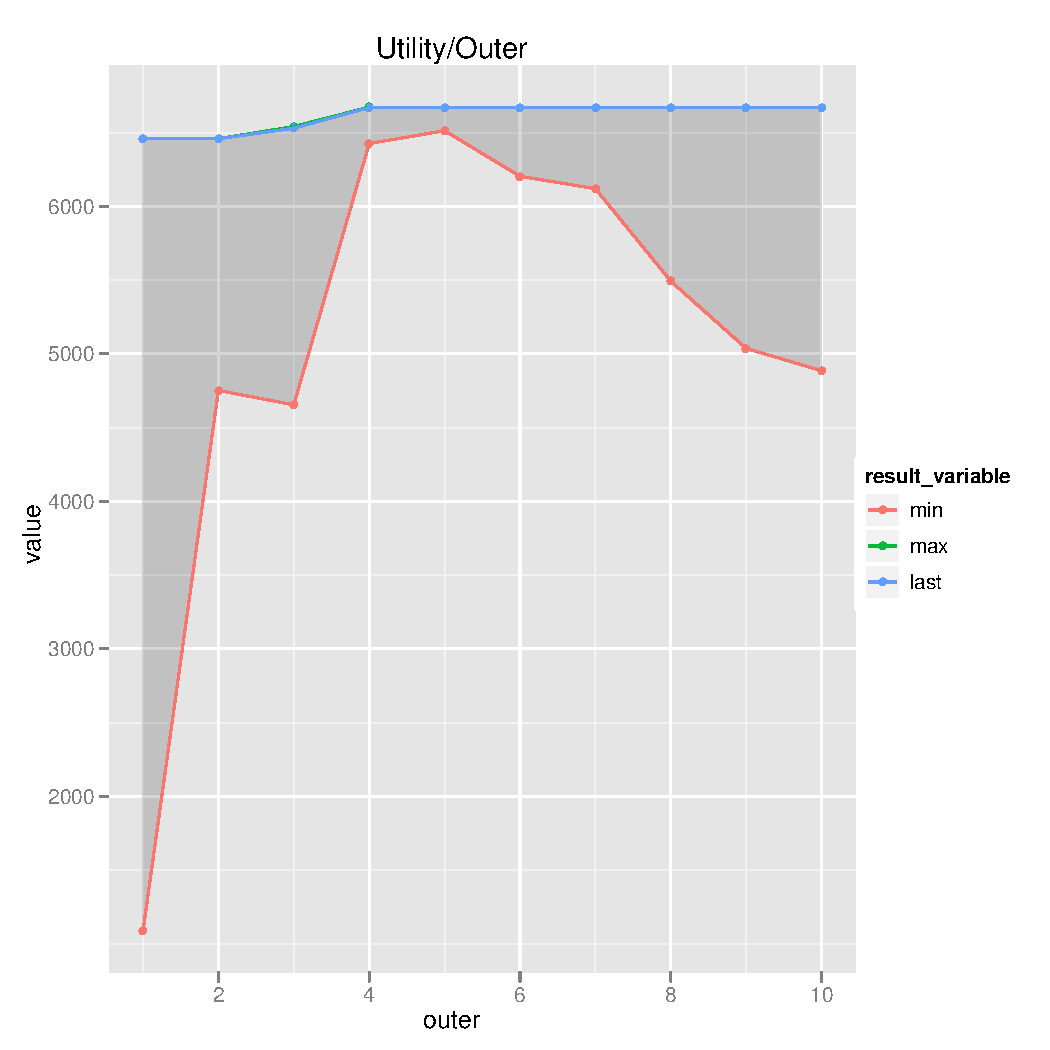
\includegraphics[width=0.8\textwidth]{exp/uncert/pres_utilouter}
  \caption{Supposed utility function in exterior loop iterations for the
    mix-problem}
  \label{pres_utilouter}
\end{figure}

Basic performance of a single run is presented in
figure~\ref{pres_utilouter}. As one can see the algorithm needs only four
iterations to reach the maximum value --- a point where no further improvement
occurs\footnote{This is not an optimal solution to the problem. By their
  nature --- intervals and scenarios of uncertainty --- a problem from this
  section does not have an optimal value.}.

Improvements of the supposed utility function and primary score are shown in
figures~\ref{pres_utilgen_01},~\ref{pres_utilgen_03} whereas the shape of the
population in fig.~\ref{pres_utilind_01},~\ref{pres_utilind_03}. One can see
that it is easy to generate a good solution to the problem --- a solution with
the best result in a given run appears in the first few generations.

Having six-dimensional objective space it is impossible to provide a section
of this space on a two-dimensional chart. However, these dimensions are not
completely independent. There is a correlation between the quantiles of the
same objective. This can be observed in fig.~\ref{pres_valweight} --- showing
the movement of population during the generation on a section of objective
space, or even better in fig.~\ref{pres_dm_choices} --- solutions marked by the
decision maker as ``good''.

As expected the solutions chosen by the DM are near the pareto-front. However,
not all of them are part of the front. Knowing that there are four other goals
besides profit$^{50\%}$ and time$^{50\%}$ explains the phenomenon.

\begin{figure}
  \centering
  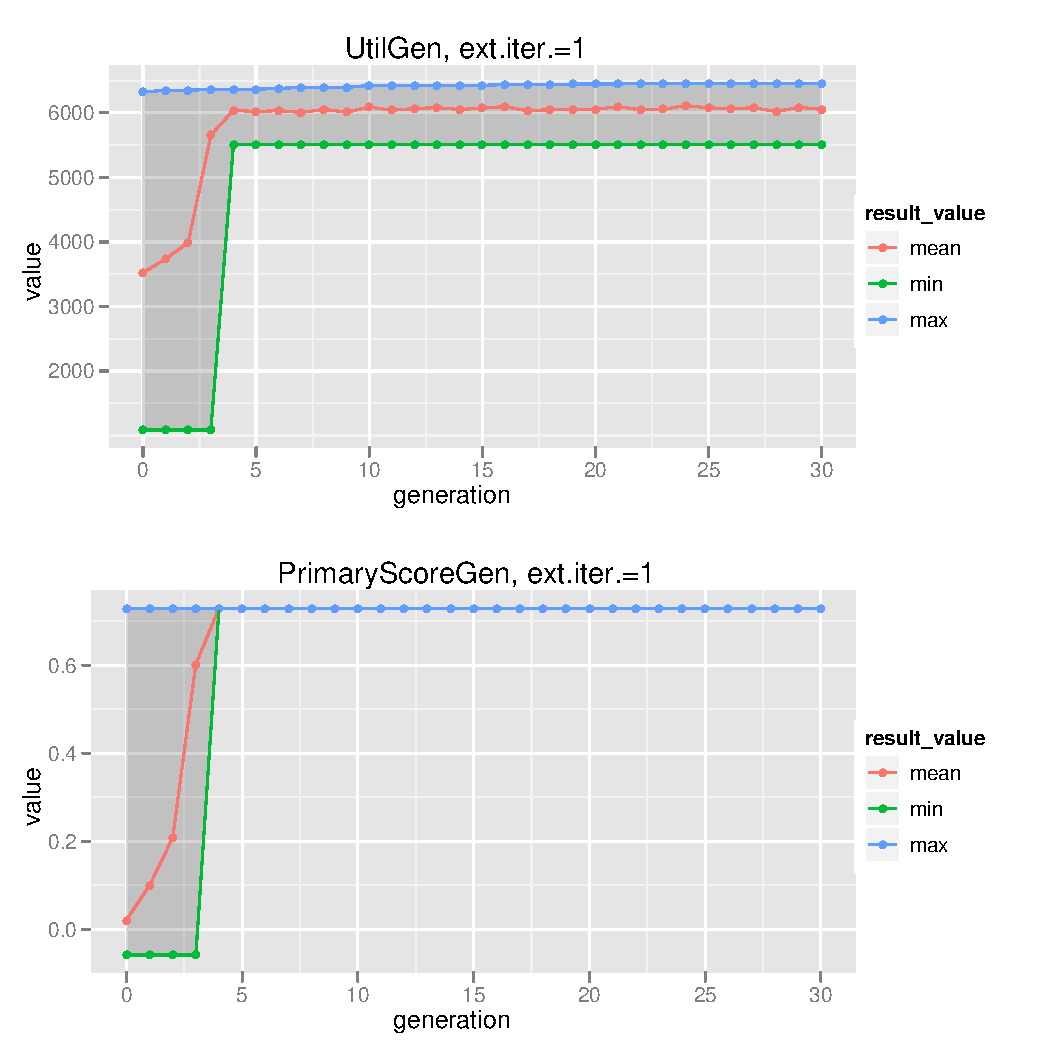
\includegraphics[width=1\textwidth]{exp/uncert/pres_utilgen_01}
  \caption{Supposed utility function and primary score improvements in an
    example run of the interior loop}
  \label{pres_utilgen_01}
\end{figure}

\begin{figure}
  \centering
  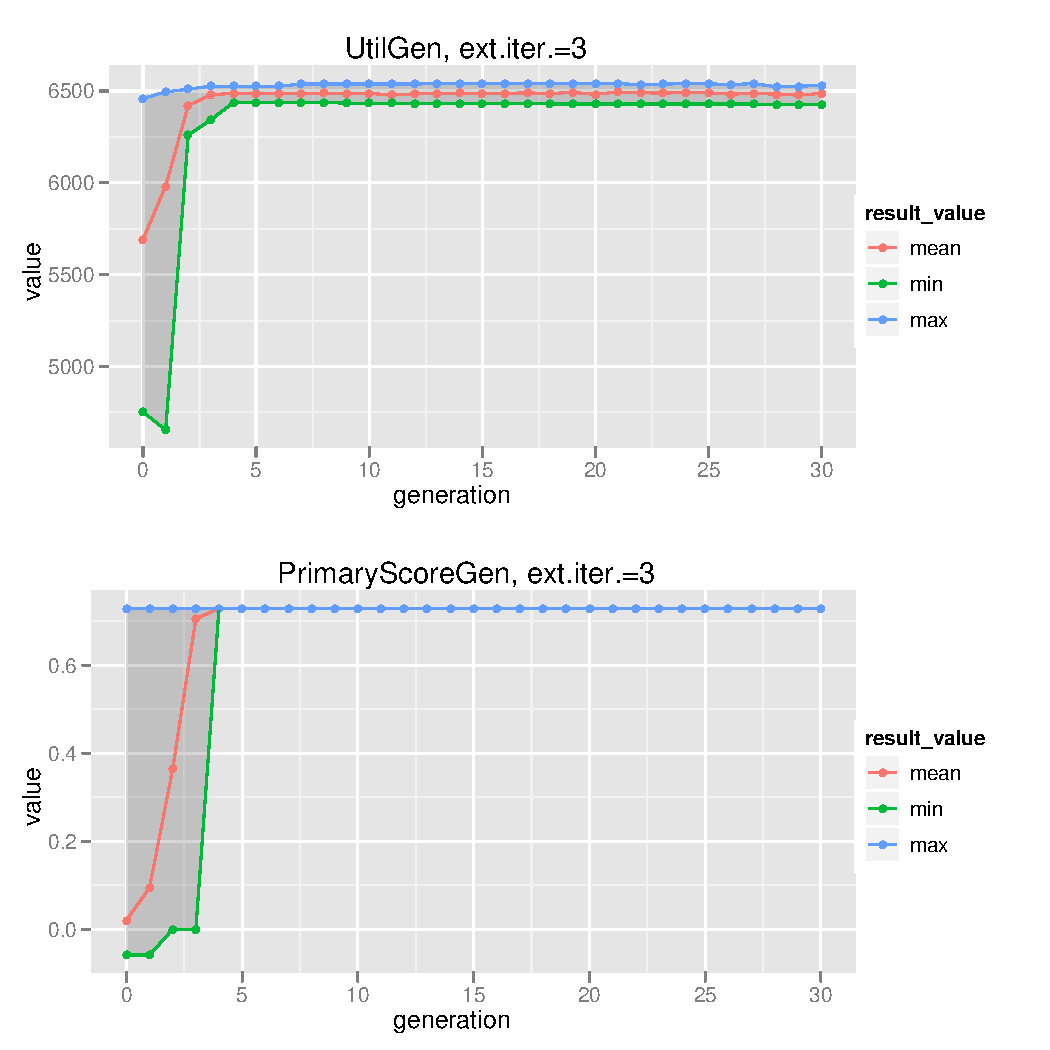
\includegraphics[width=1\textwidth]{exp/uncert/pres_utilgen_03}
  \caption{Supposed utility function and primary score improvements in an example run of the
    interior loop}
  \label{pres_utilgen_03}
\end{figure}

\begin{figure}
  \centering
  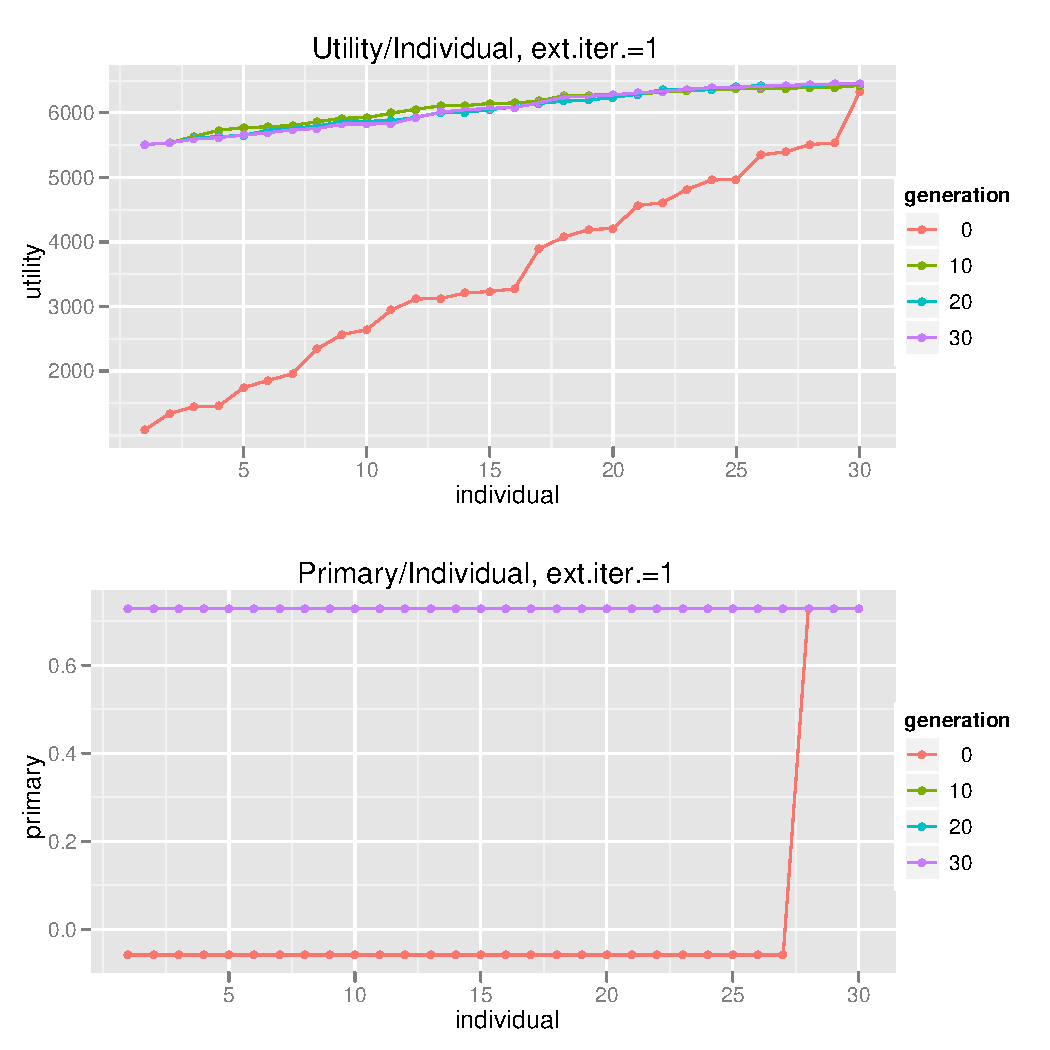
\includegraphics[width=1\textwidth]{exp/uncert/pres_utilind_01}
  \caption{Changes of the population shape in an example run of the interior
    loop}
  \label{pres_utilind_01}
\end{figure}

\begin{figure}
  \centering
  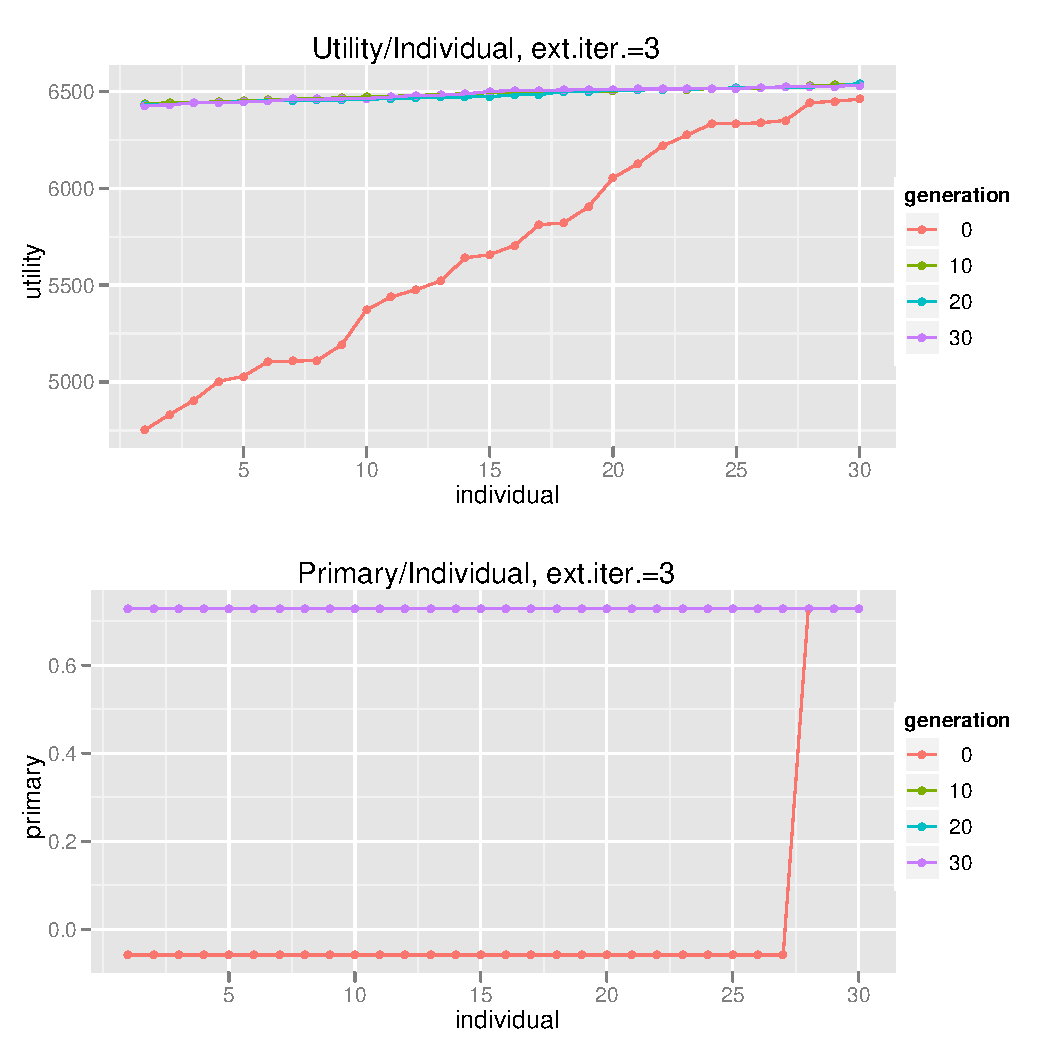
\includegraphics[width=1\textwidth]{exp/uncert/pres_utilind_03}
  \caption{Changes of the population shape in an example run of the interior
    loop}
  \label{pres_utilind_03}
\end{figure}

\begin{figure}
  \centering
  \makebox[\textwidth]{
    \subfloat{
      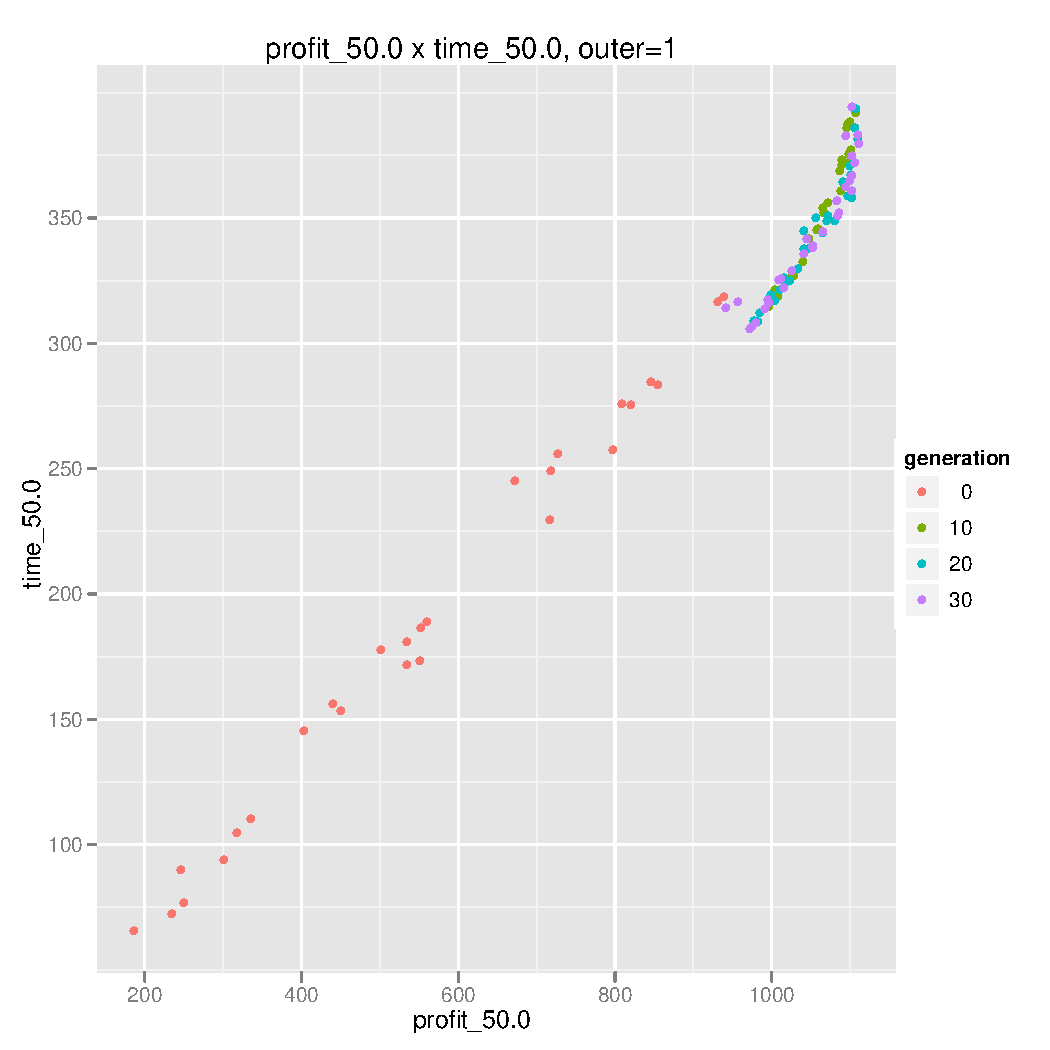
\includegraphics[scale=0.53]{exp/uncert/pres_valweight_01}
      \label{pres_valweight_01}
    }
    \subfloat{
      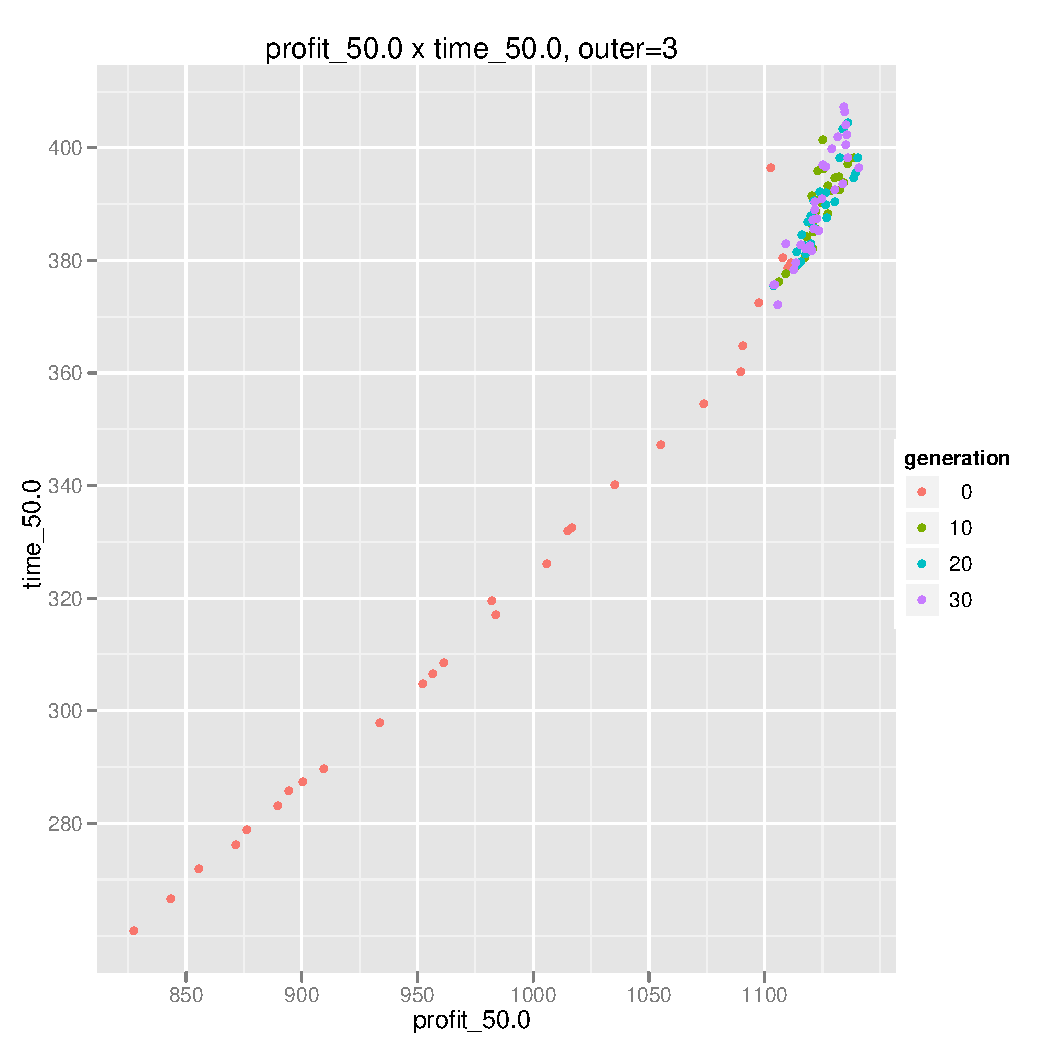
\includegraphics[scale=0.53]{exp/uncert/pres_valweight_03}
      \label{pres_valweight_03}
    }
  }
  \caption{Two-dimensional section of the objective space}
  \label{pres_valweight}
\end{figure}

\begin{figure}
  \centering
  \makebox[\textwidth]{
    \subfloat{
      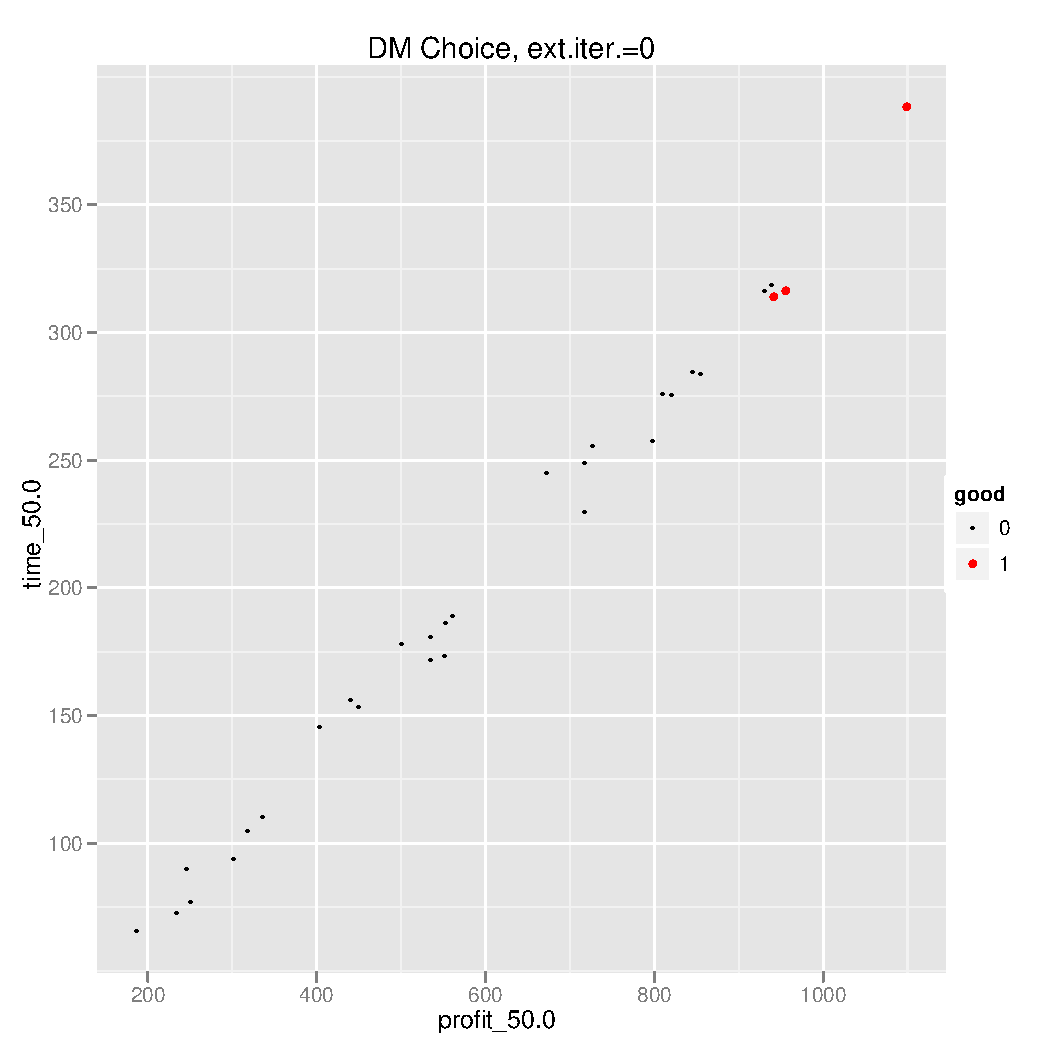
\includegraphics[scale=0.53]{exp/uncert/pres_dm_choices_01}
      \label{pres_dm_choices_01}
    }
    \subfloat{
      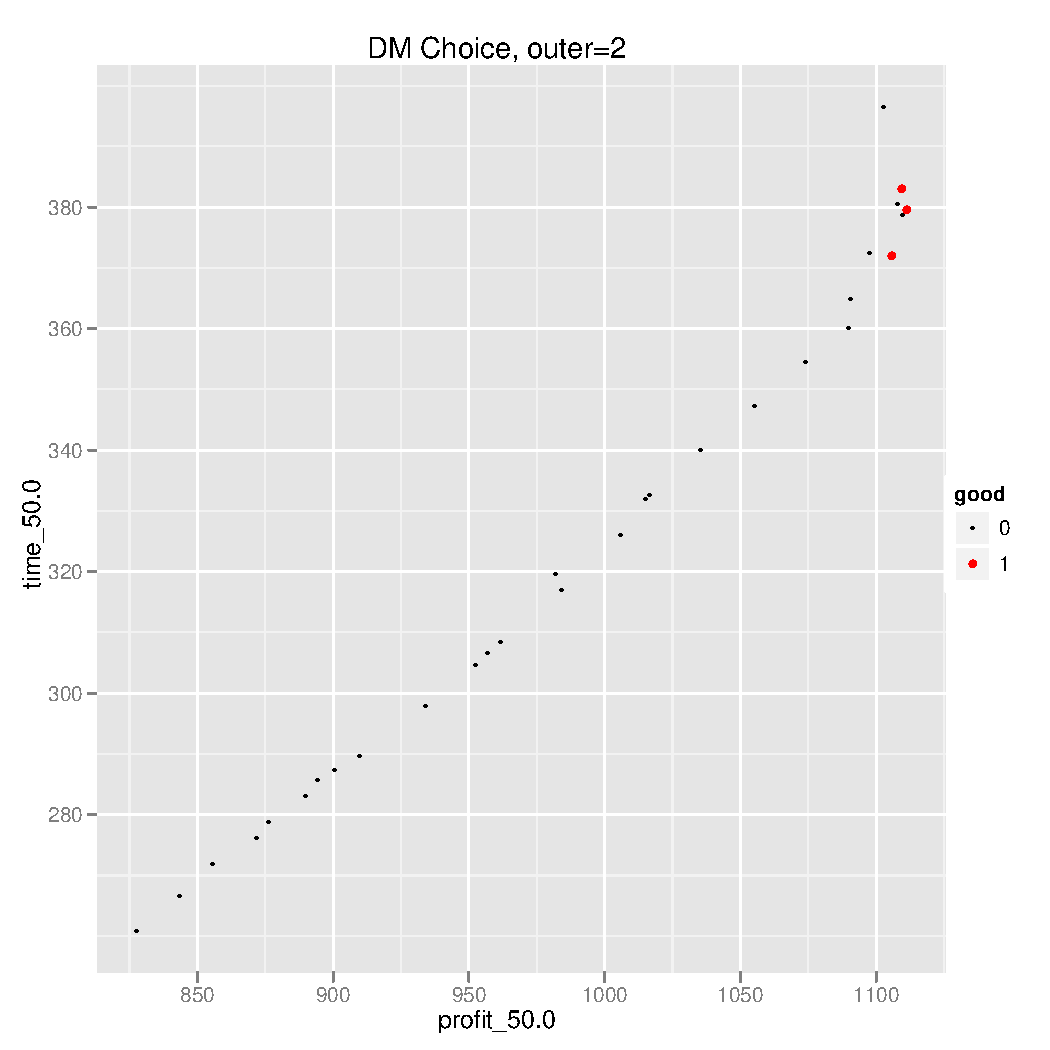
\includegraphics[scale=0.53]{exp/uncert/pres_dm_choices_03}
      \label{pres_dm_choices_03}
    }
  }
  \caption{Two-dimensional section of the objective space}
  \label{pres_dm_choices}
\end{figure}
\clearpage{}

\subsection{The performance on exemplary problems}
To see how well DARWIN can infer the decision maker's preferences a comparison
with the supposed utility function is given. For this section the experiments
were performed on all exemplary problems with interval coefficients --- mix
problem (also labeled as presentation problem), dtlz1 (version with four and
ten criteria) and dtlz7.

The problems were solved with default (base) values of configuration options
as well as with an increased number of generations (from $30$ to $60$). Tests
whose names end with \texttt{\_rules} are using primary and secondary score;
tests with names ending with \texttt{\_supp} are using the supposed utility
function value as an objective in evolutionary optimization.

\begin{figure}
  \centering
  \makebox[\textwidth]{
    \subfloat{
      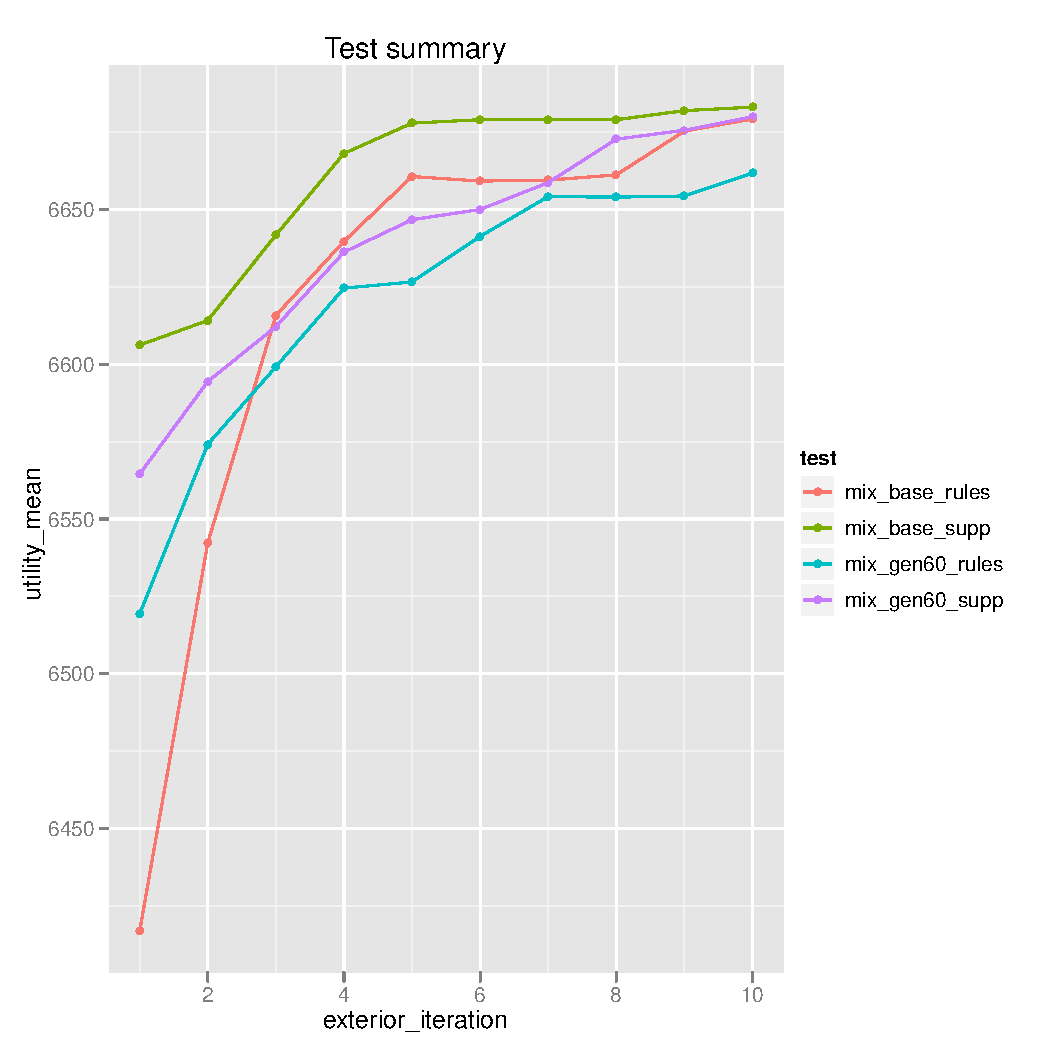
\includegraphics[scale=0.53]{exp/uncert/pres_perf1}
      \label{pres_perf1}
    }
    \subfloat{
      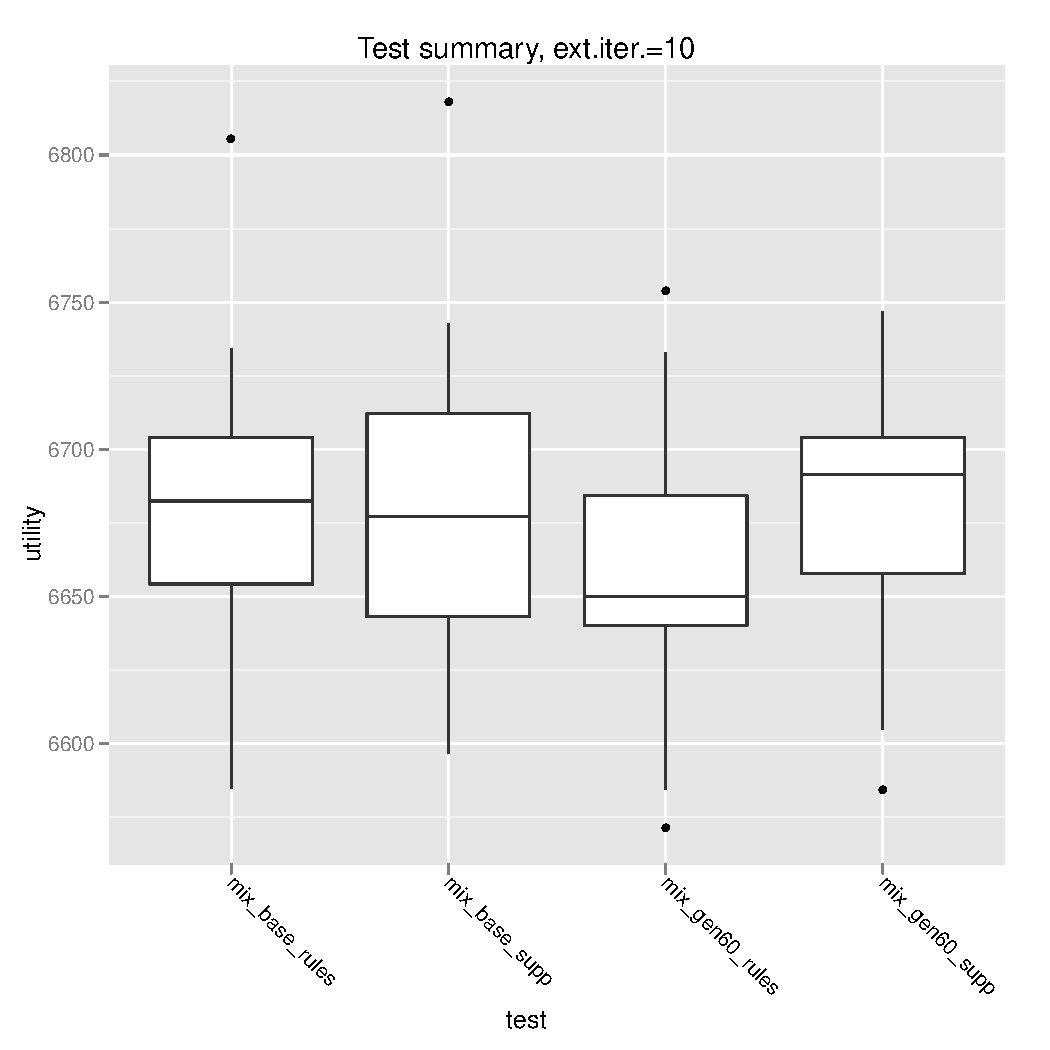
\includegraphics[scale=0.53]{exp/uncert/pres_perf1b}
      \label{pres_perf1b}
    }
  }
  \caption{Performance comparison on the mix problem}
  \label{pres_perf}
\end{figure}

\begin{figure}
  \centering
  \makebox[\textwidth]{
    \subfloat{
      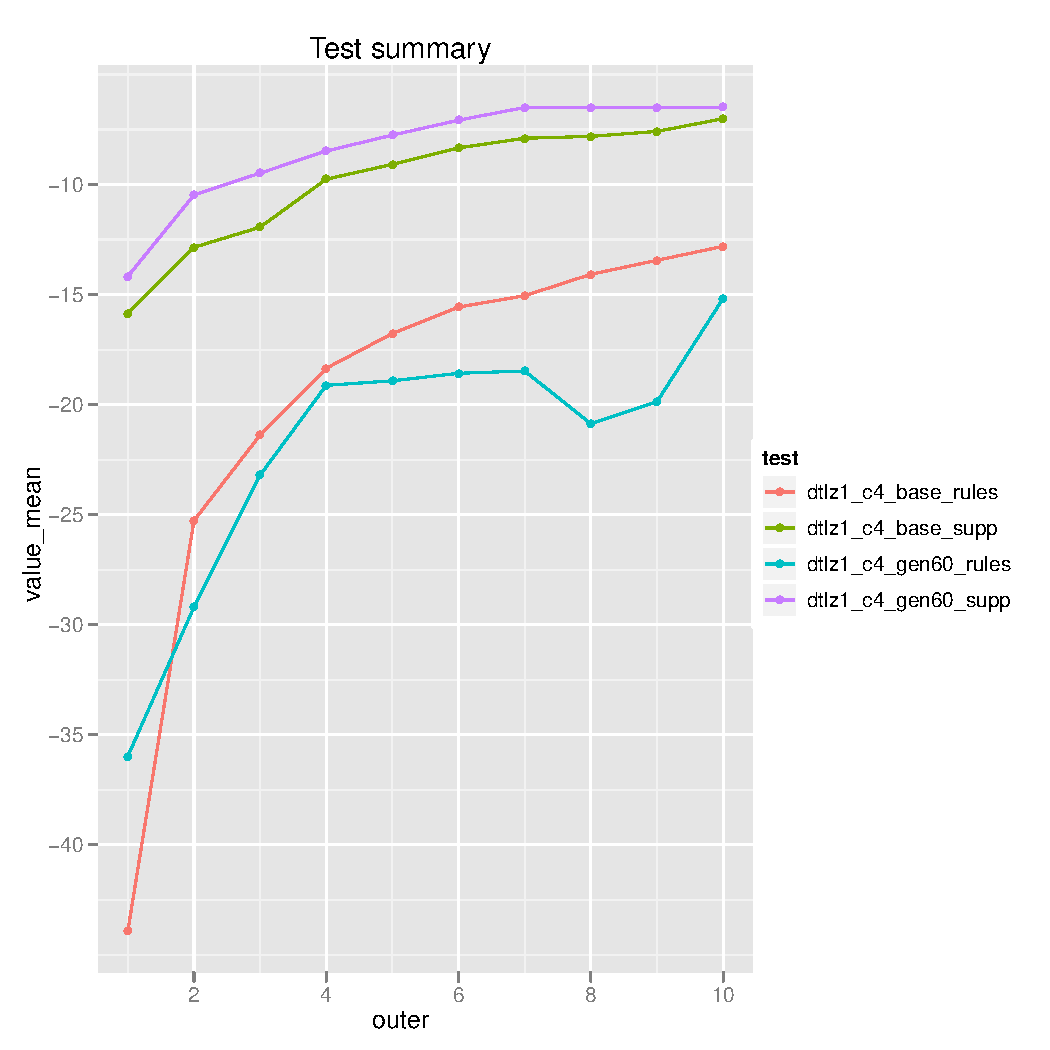
\includegraphics[scale=0.53]{exp/uncert/dtlz1_c4_perf1}
      \label{dtlz1_c4_perf1}
    }
    \subfloat{
      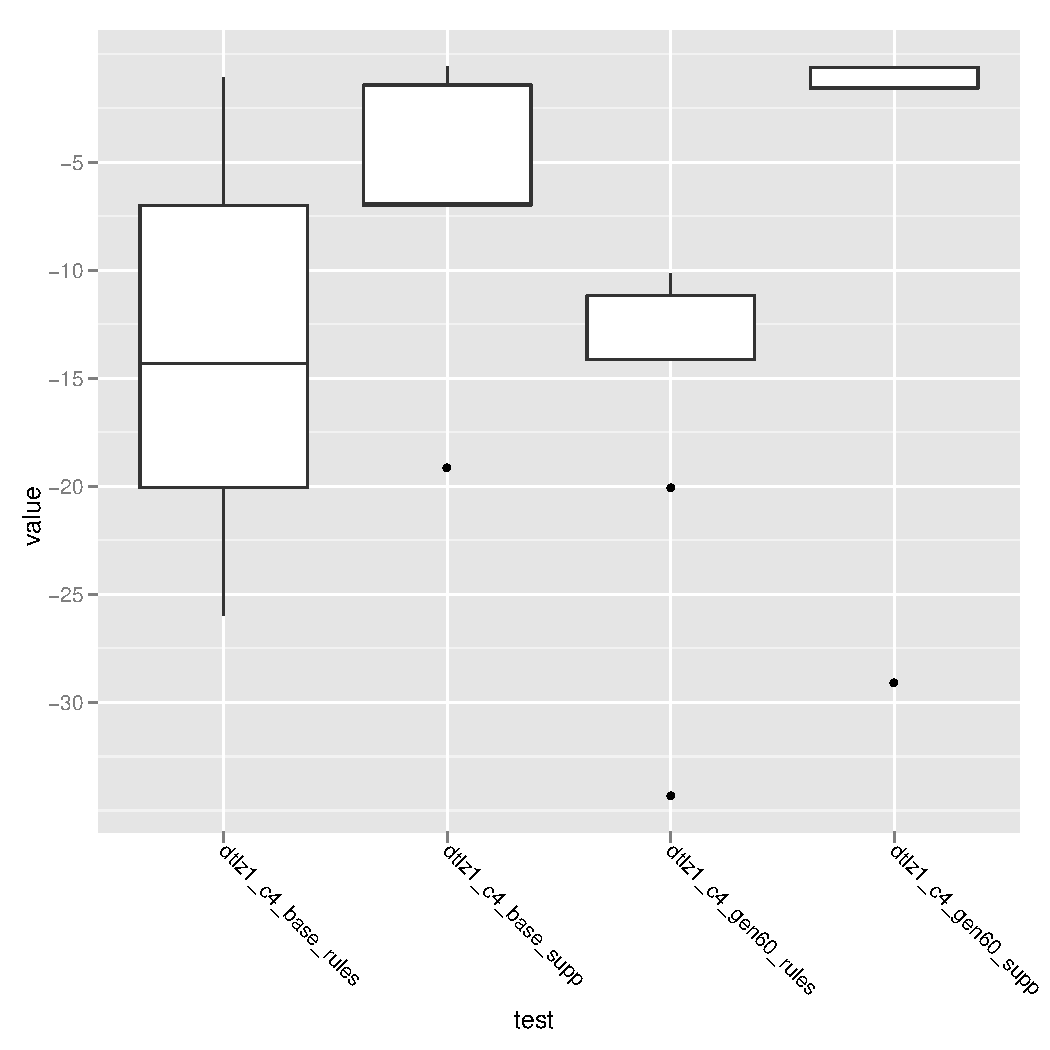
\includegraphics[scale=0.53]{exp/uncert/dtlz1_c4_perf1b}
      \label{dtlz1_c4_perf1b}
    }
  }
  \caption{Performance comparison on the four-criteria DTLZ1 problem}
  \label{dtlz1_c4_perf}
\end{figure}

\begin{figure}
  \centering
  \makebox[\textwidth]{
    \subfloat{
      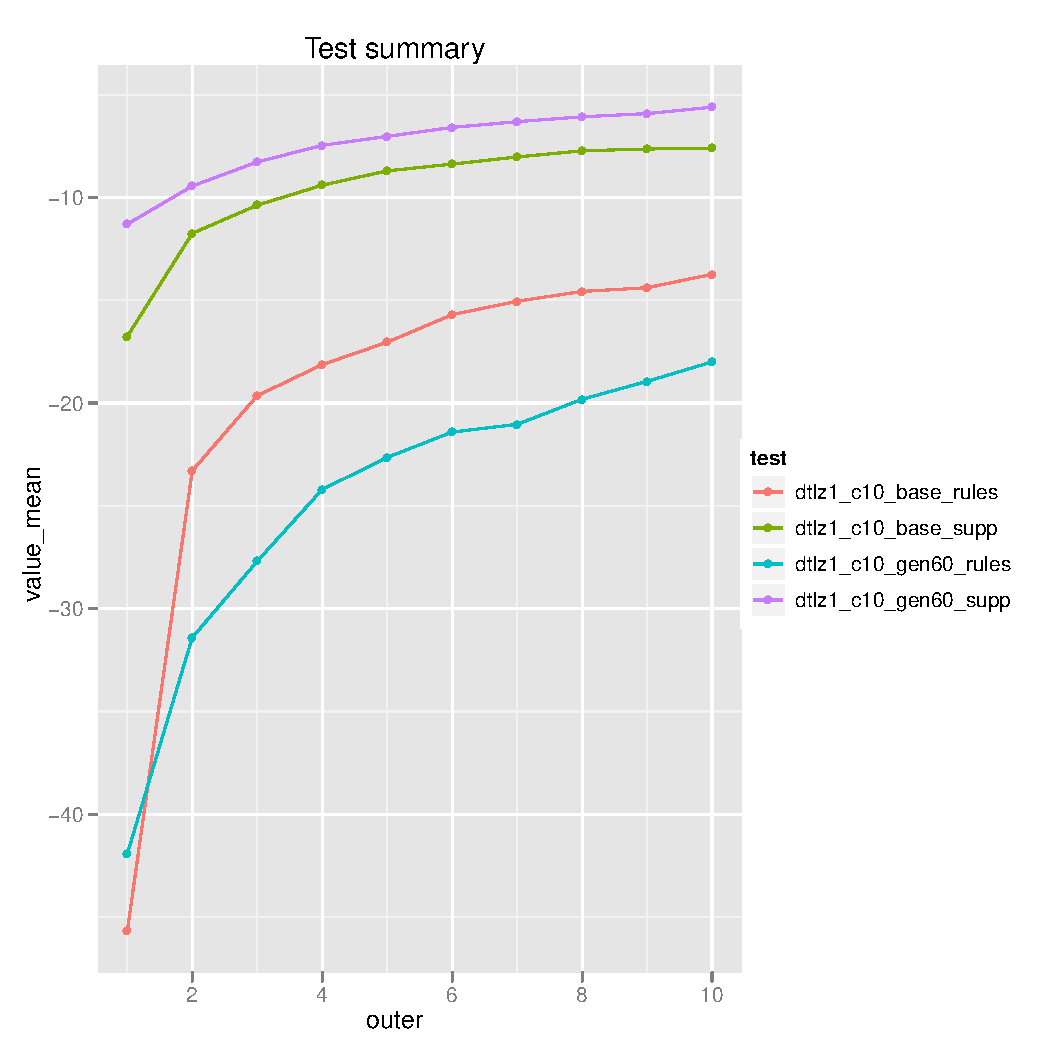
\includegraphics[scale=0.53]{exp/uncert/dtlz1_c10_perf1}
      \label{dtlz1_c10_perf1}
    }
    \subfloat{
      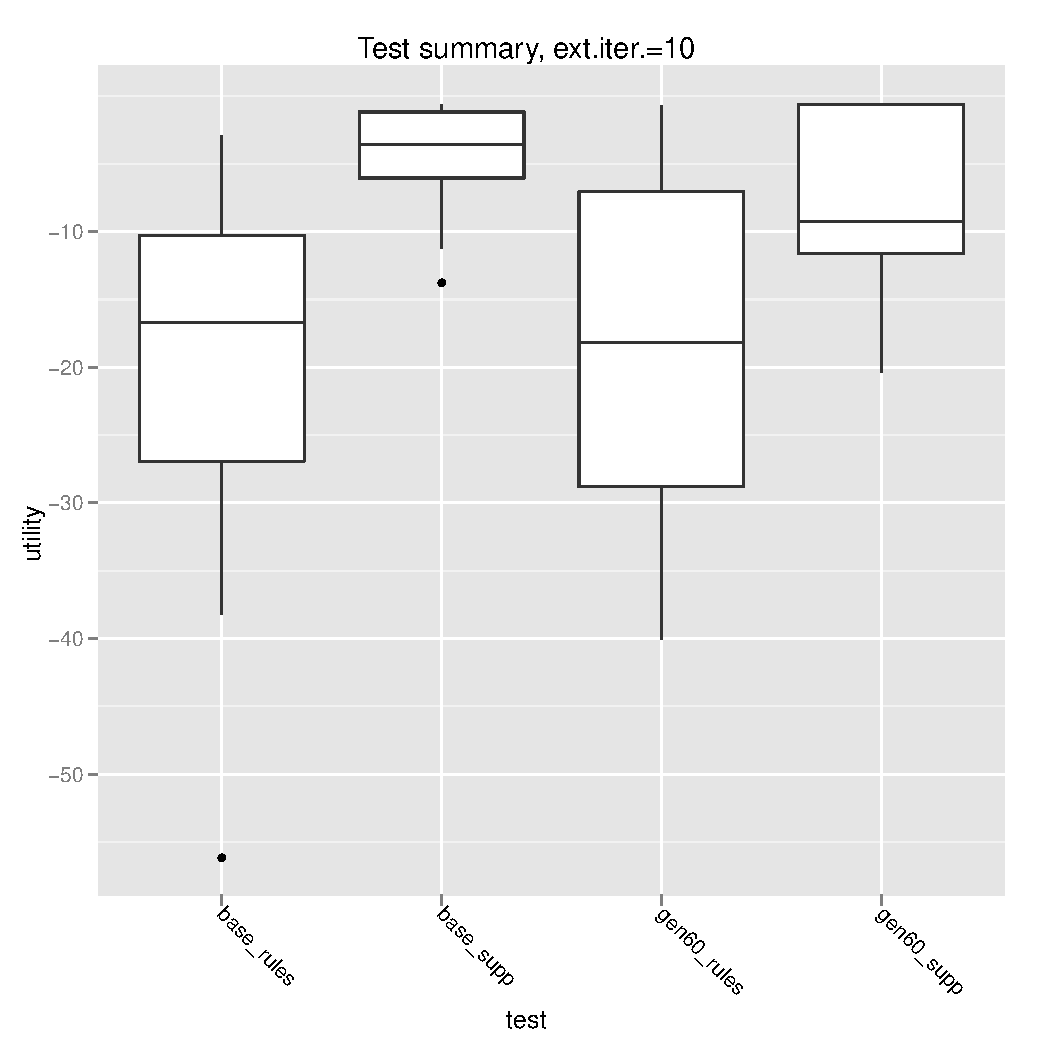
\includegraphics[scale=0.53]{exp/uncert/dtlz1_c10_perf1b}
      \label{dtlz1_c10_perf1b}
    }
  }
  \caption{Performance comparison on the ten-criteria DTLZ1 problem}
  \label{dtlz1_c10_perf}
\end{figure}

\begin{figure}
  \centering
  \makebox[\textwidth]{
    \subfloat{
      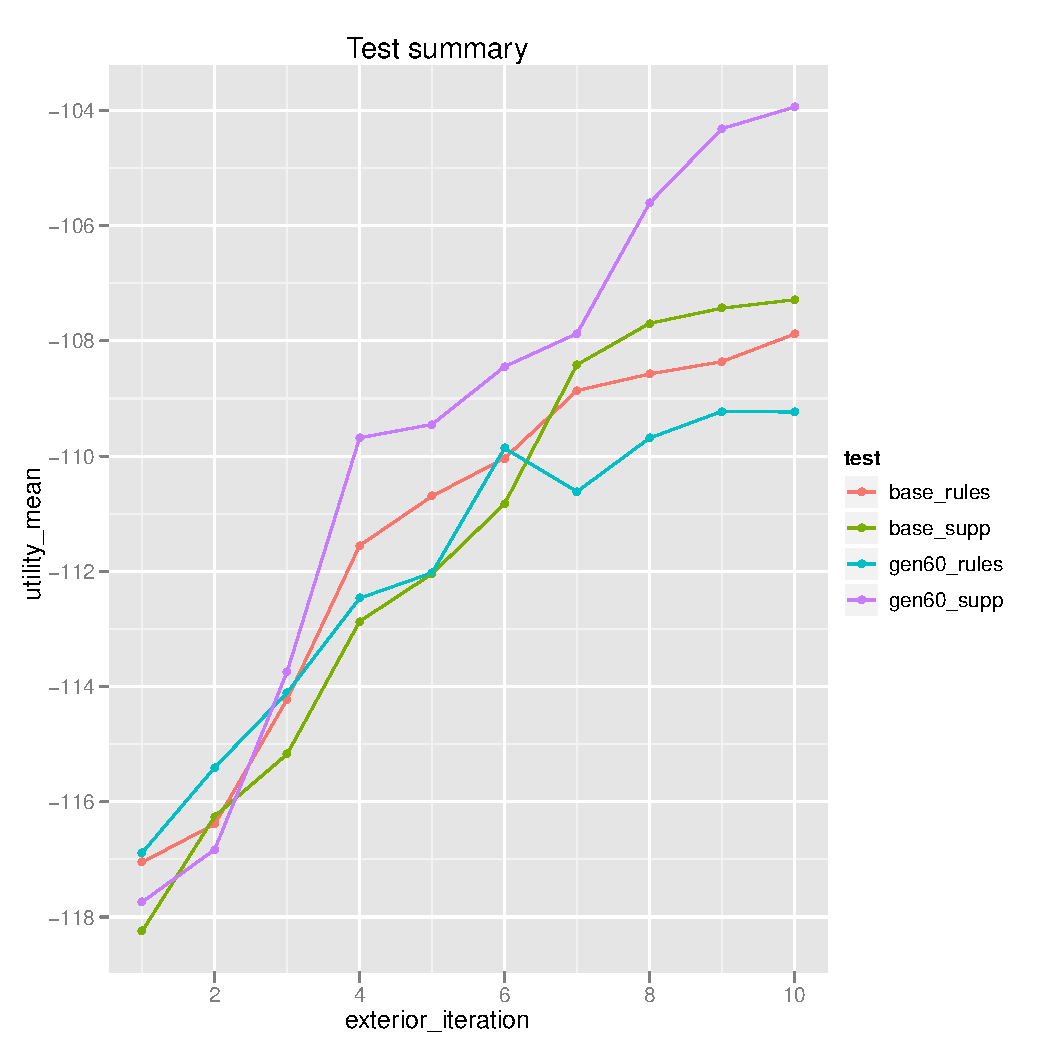
\includegraphics[scale=0.53]{exp/uncert/dtlz7_c4_perf1}
      \label{dtlz7_c4_perf1}
    }
    \subfloat{
      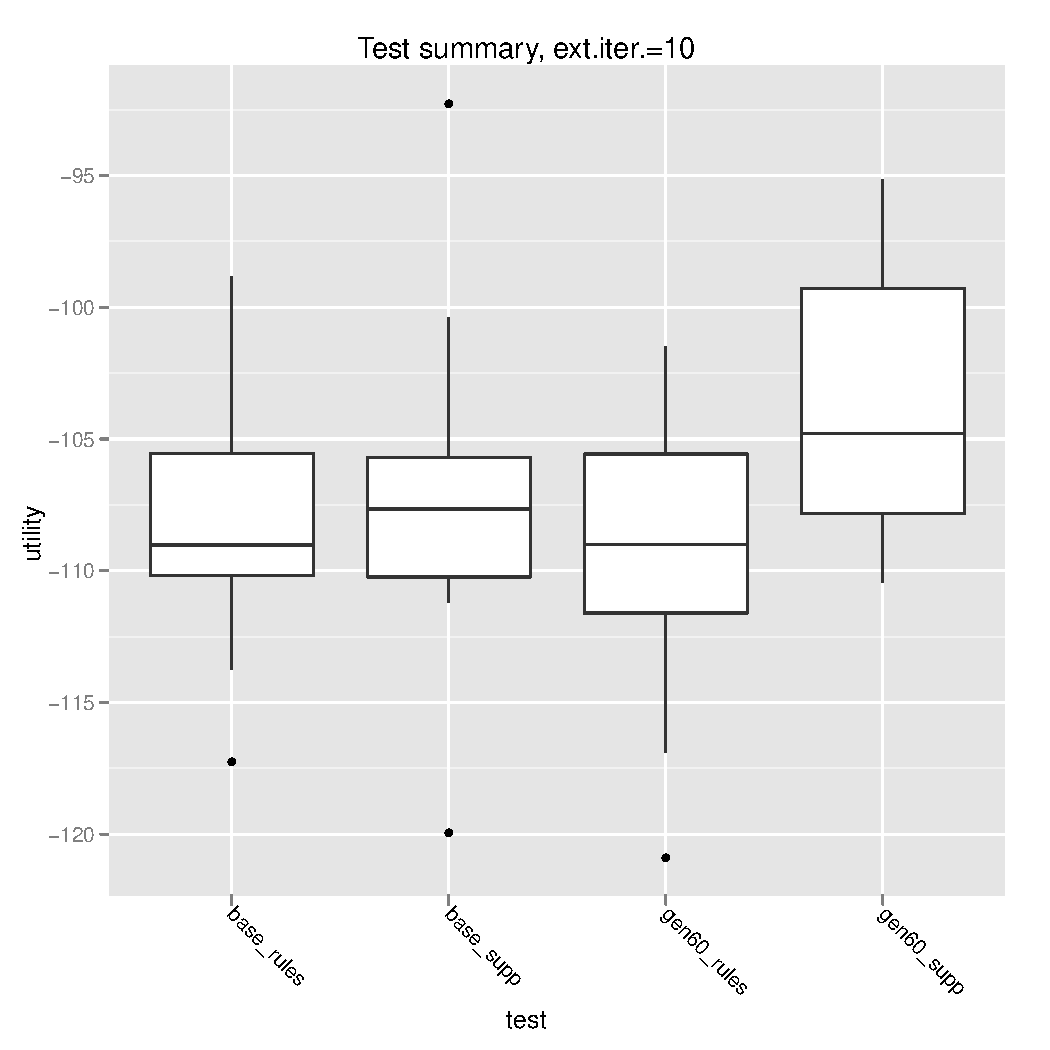
\includegraphics[scale=0.53]{exp/uncert/dtlz7_c4_perf1b}
      \label{dtlz7_c4_perf1b}
    }
  }
  \caption{Performance comparison on the four-criteria DTLZ7 problem}
  \label{dtlz7_c4_perf}
\end{figure}

\begin{table}
  \centering
  \begin{tabular}{r c c c}
    \hline
    test \ optimization & supposed & rules & distance \\
    \hline
    \hline
    mix\_base & 6683.14 & 6678.95 & 0.06\% \\
    mix\_gen60 & 6680.05 & 6661.41 & 0.28\% \\
    dtlz1\_c4\_base & 7.01 & 12.81 & 45.29\% \\
    dtlz1\_c4\_gen60 & 6.48 & 15.18 & 57.28\% \\
    dtlz1\_c10\_base & 7.60 & 13.73 & 44.68\% \\
    dtlz1\_c10\_gen60 & 5.61 & 18.00 & 68.85\% \\
    dtlz7\_c4\_base & 104.72 & 108.74 & 3.69\% \\
    dtlz7\_c4\_gen60 & 104.95 & 110.28 & 4.83\% \\
    \hline
  \end{tabular}
  \caption{Performance comparison on robust multi-objective problems}
  \label{t:perf-comp}
\end{table}

The results are shown in table~\ref{t:perf-comp} and presented in
figure~\ref{pres_perf}, \ref{dtlz1_c4_perf}, \ref{dtlz1_c10_perf}
and~\ref{dtlz7_c4_perf}. There was almost no difference for the mix problem
(less than $1\%$) and a minor difference for the dtlz7 problem --- less than
$5\%$. Unfortunately, differences for dtlz1 problems (both four- and
ten-criteria) were important and noticeable --- about $50\%$ percent after ten
iterations. \textcolor{red}{The result for dtlz1 are far below the
  expectations --- the default parameters are not appropriate for the
  problem. A~better result here is still possible, however it requires
  a~tuning of the parameters (see~[inref]).}

 \clearpage{}

\subsection{The influence of parameters on the method}

The importance of basic parameters was evaluated again in the robust
environment. The numerical results are presented in the
table~\ref{t:base2_imp_1} and~\ref{t:base2_imp_2}. Also charts are included to
visualize the relations (fig.~\ref{params}).

Unfortunately, no clear pattern emerges. For a mix problem the solution is
robust --- changing the basic parameters changes the value of the result no
more than a $1\%$ after ten iterations.For the DTLZ7 problem the situation is
similar --- differences are bigger now, however still less than $5\%$.

Differences are bigger and important for the DTLZ1 problems (four- and
ten-criteria). However, the standard deviations are of the same order of
magnitude as mean values of the results. So one should say the results are
inconclusive here and it is impossible to make a suggestion based solely on
these results.

\begin{table}[htb]
  \centering
  \begin{tabular}{r c c c c c c}
    & \multicolumn{3}{c}{Mix problem} & \multicolumn{3}{c}{DTLZ1 c4} \\
    \hline
    test & mean & sd & improvement & mean & sd & improvement \\
    \hline
    \hline
    base & 6665.60 & 57.27 & 0.00\% & -9.99 & 6.83 & 0.00\% \\
    generation45 & 6661.72 & 47.52 & -0.06\% & -16.04 & 12.47 & 60.63\% \\
    generation60 & 6661.14 & 45.08 & -0.07\% & -9.63 & 7.78 & -3.61\% \\
    scenario45 & 6617.60 & 47.33 & -0.72\% & -13.12 & 11.37 & 31.34\% \\
    scenario60 & 6639.54 & 33.98 & -0.39\% & -13.95 & 8.50 & 39.68\% \\
    solution45 & 6705.68 & 52.96 & 0.60\% & -10.43 & 8.33 & 4.44\% \\
    solution60 & 6685.43 & 56.78 & 0.30\% & -11.68 & 8.23 & 16.97\% \\
    \hline
  \end{tabular}
  \caption{Importance of base parameters in robust environment}
  \label{t:base2_imp_1}
\end{table}

\begin{table}[htb]
  \centering
  \begin{tabular}{r c c c c c c}
    & \multicolumn{3}{c}{DTLZ1 c10} & \multicolumn{3}{c}{DTLZ7 c4} \\
    \hline
    test & mean & sd & improvement & mean & sd & improvement \\
    \hline
    \hline
    base & -15.30 & 11.20 & 0.00\% & -109.23 & 5.87 & 0.00\% \\
    generation45 & -15.92 & 13.27 & 4.03\% & -109.23 & 6.96 & 0.00\% \\
    generation60 & -21.63 & 12.55 & 41.37\% & -108.33 & 10.87 & -0.82\% \\
    scenario45 & -17.32 & 11.15 & 13.17\% & -111.98 & 5.34 & 2.52\% \\
    scenario60 & -16.67 & 13.30 & 8.91\% & -112.54 & 3.45 & 3.03\% \\
    solution45 & -13.89 & 9.63 & -9.22\% & -107.88 & 6.39 & -1.23\% \\
    solution60 & -9.55 & 6.81 & -37.62\% & -109.98 & 6.37 & 0.69\% \\
    \hline
  \end{tabular}
  \caption{Importance of base parameters in robust environment}
  \label{t:base2_imp_2}
\end{table}

\begin{figure}
  \centering
  \makebox[\textwidth]{
    \subfloat[Mix problem]{
      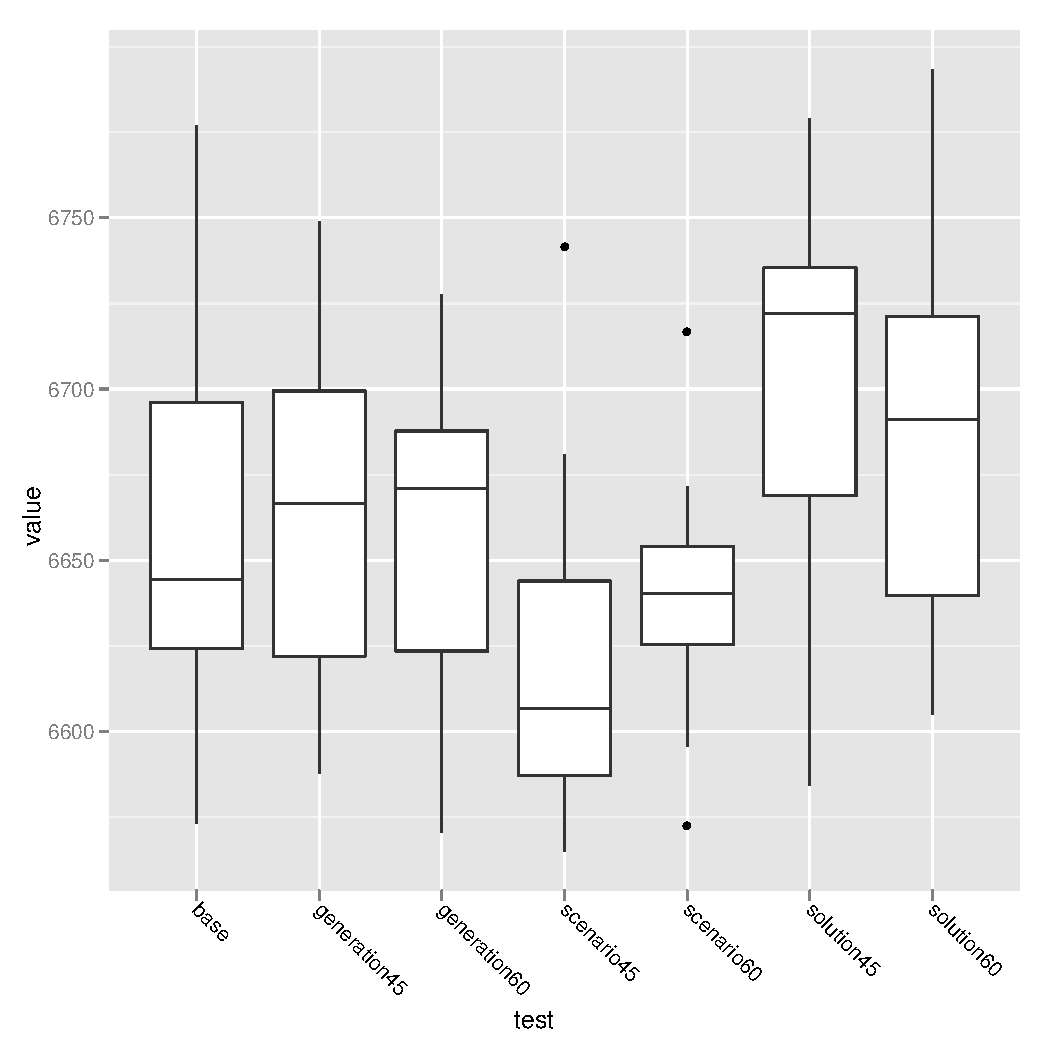
\includegraphics[scale=0.53]{exp/uncert/pres_params}
      \label{pres_params}
    }
    \subfloat[DTLZ1 four criteria]{
      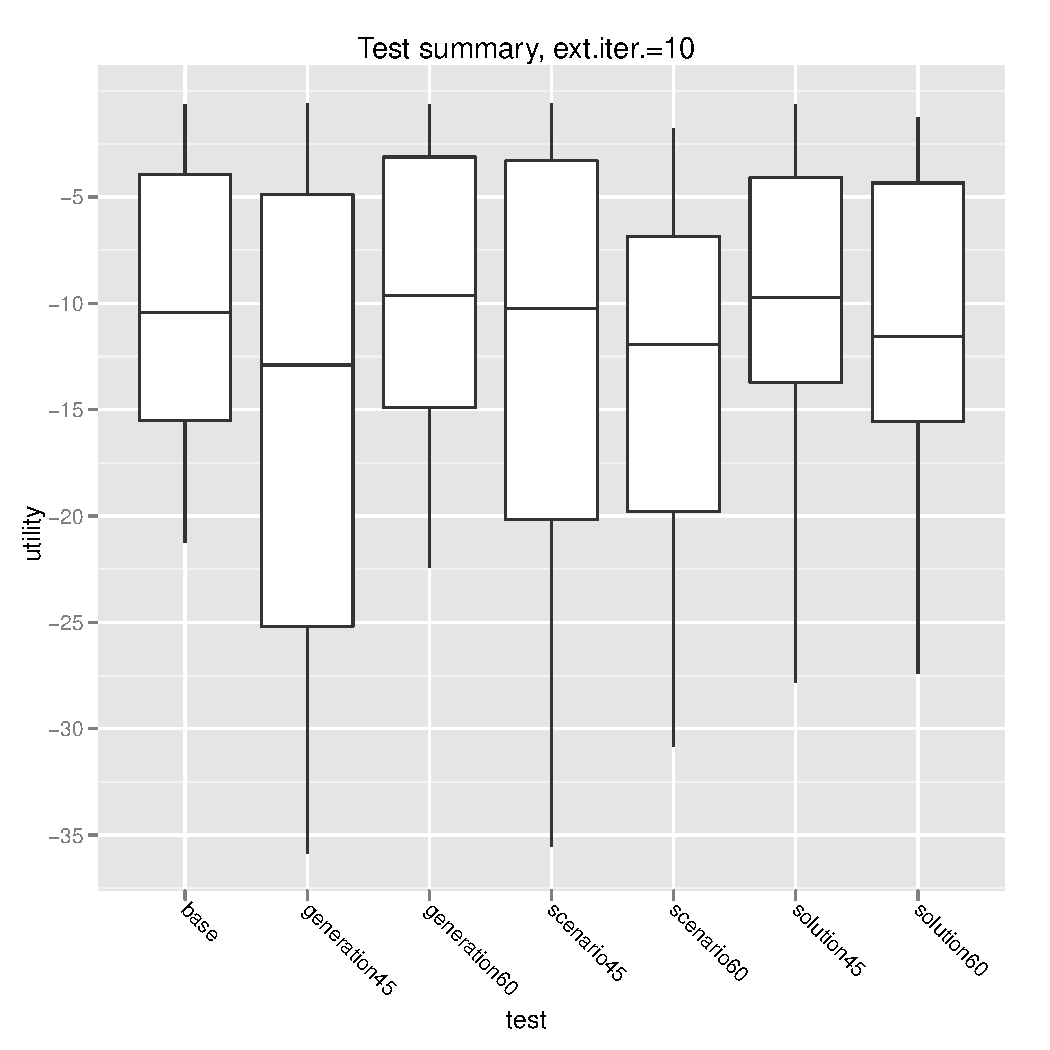
\includegraphics[scale=0.53]{exp/uncert/dtlz1_c4_params}
      \label{dtlz1_c4_params}
    }
  }
  \makebox[\textwidth]{
    \subfloat[DTLZ1 ten criteria]{
      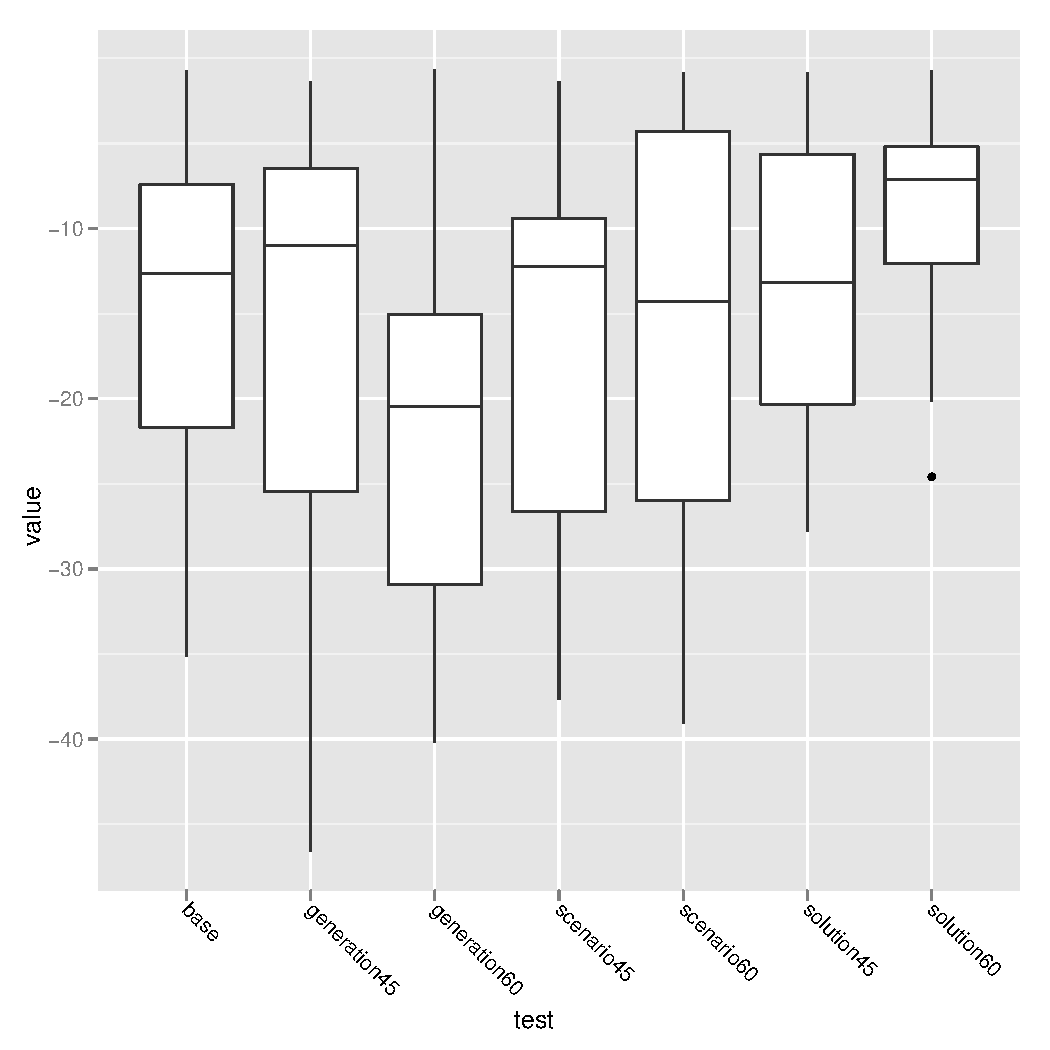
\includegraphics[scale=0.53]{exp/uncert/dtlz1_c10_params}
      \label{dtlz1_c10_params}
    }
    \subfloat[DTLZ7 four criteria]{
      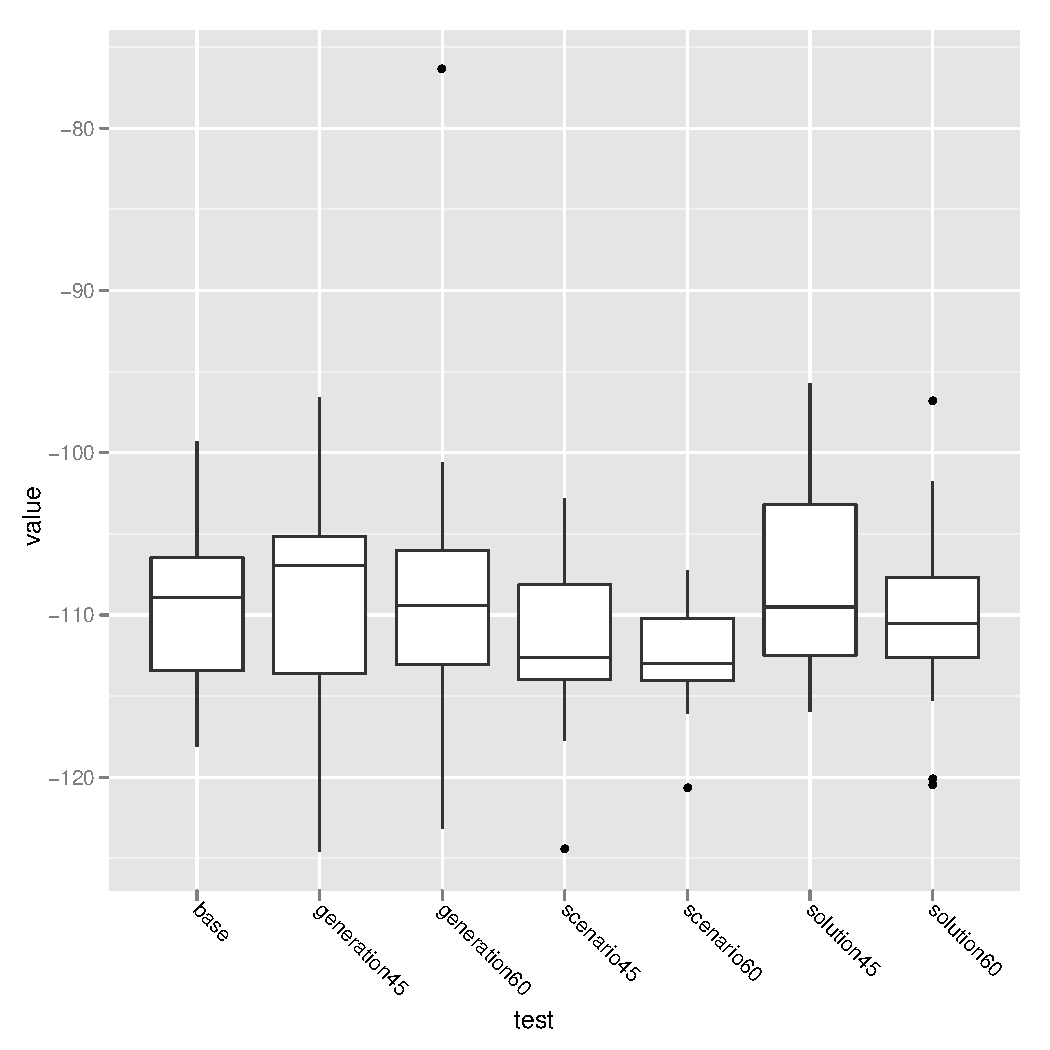
\includegraphics[scale=0.53]{exp/uncert/dtlz7_c4_params}
      \label{dtlz7_c4_params}
    }
  }
  \caption{Effect of params in DM's decisions}
  \label{params}
\end{figure}

\clearpage{}

\subsection{Noise in the DM's decisions}

In order to check the impact of a noise in DM's decisions, experiments were
performed. The results are presented in figure~\ref{noise} and in the
tables~\ref{t:un_noise_1} and~\ref{t:un_noise_2}.

Again one has to analyze the results excluding the DTLZ1 problem. This is
because of the standard deviation of the series of results --- again it is the
same order of magnitude as the value itself.

In the Mix and DTLZ7 problems the effect of the noise starts to be an
important factor only in case of medium- (noise$_5$) --- the results differ
about $8\%$ and in case of a major-noise (noise$_6$) --- difference about 12\%
for the mix problem and about 8\% for the DTLZ7 problem.

The situation is similar to the impact on problems defined without
uncertainty. Even if one adds the interval coefficients to the problem, the
solution is still robust with respect to the noise.


\begin{figure}
  \centering
  \makebox[\textwidth]{
    \subfloat[Mix problem]{
      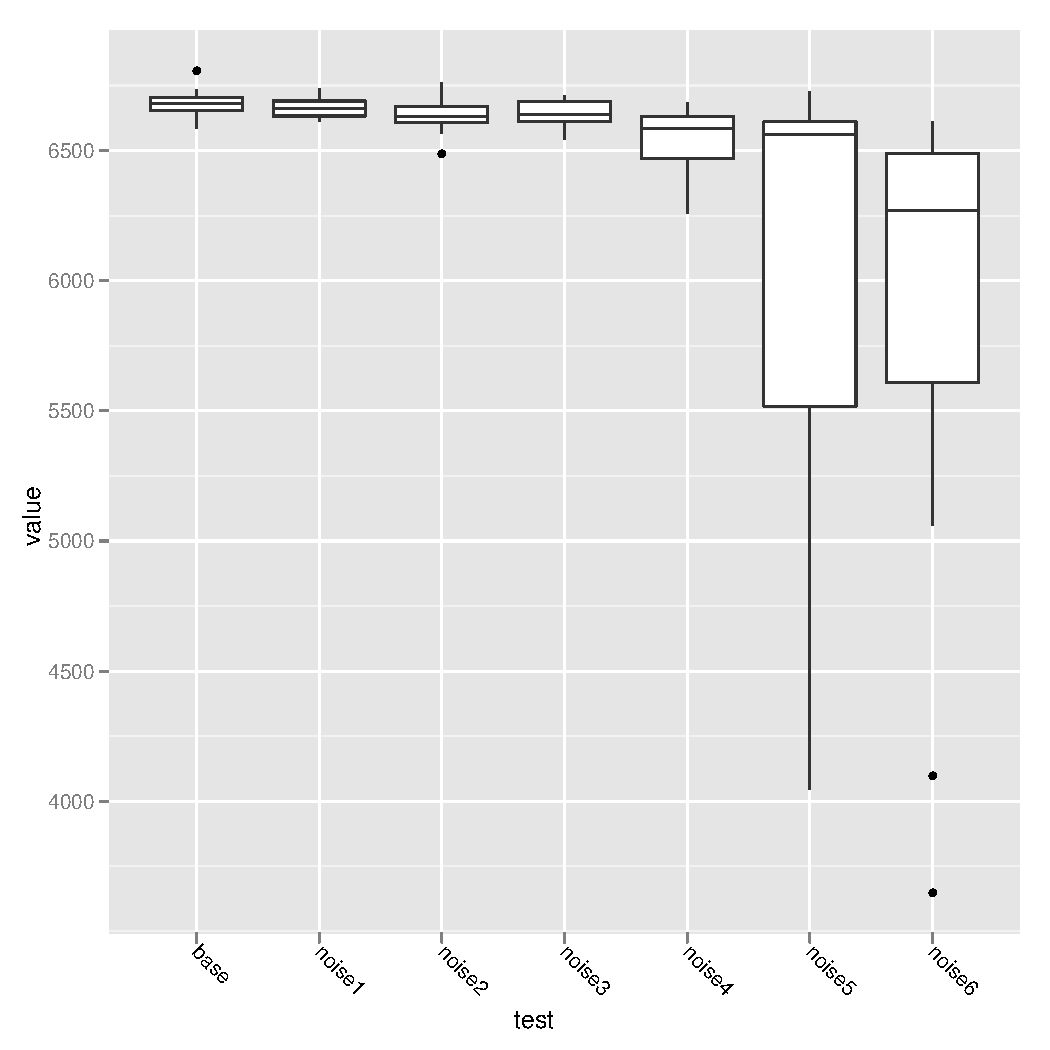
\includegraphics[scale=0.53]{exp/uncert/pres_noise}
      \label{pres_noise}
    }
    \subfloat[DTLZ1 four-criteria]{
      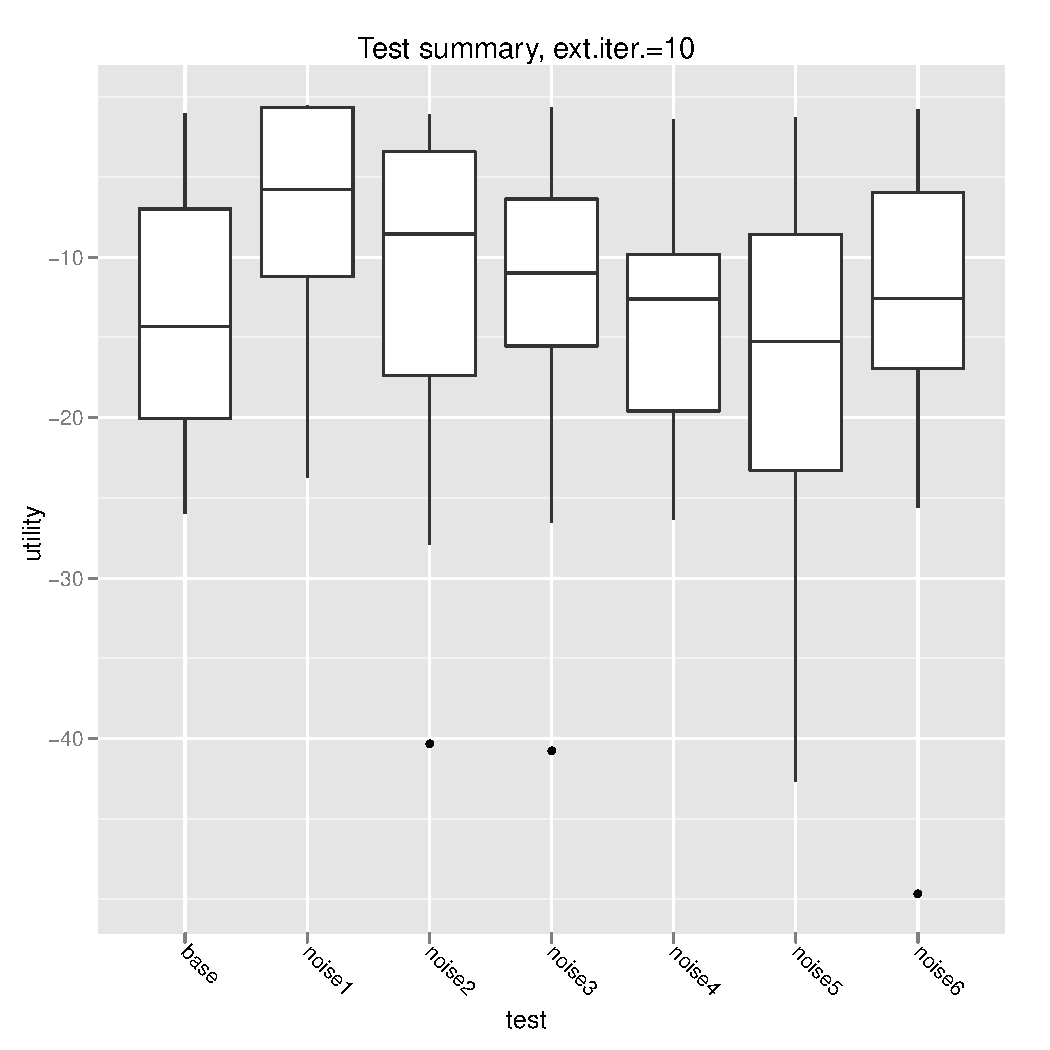
\includegraphics[scale=0.53]{exp/uncert/dtlz1_c4_noise}
      \label{dtlz1_c4_noise}
    }
  }
  \makebox[\textwidth]{
    \subfloat[DTLZ1 ten-criteria]{
      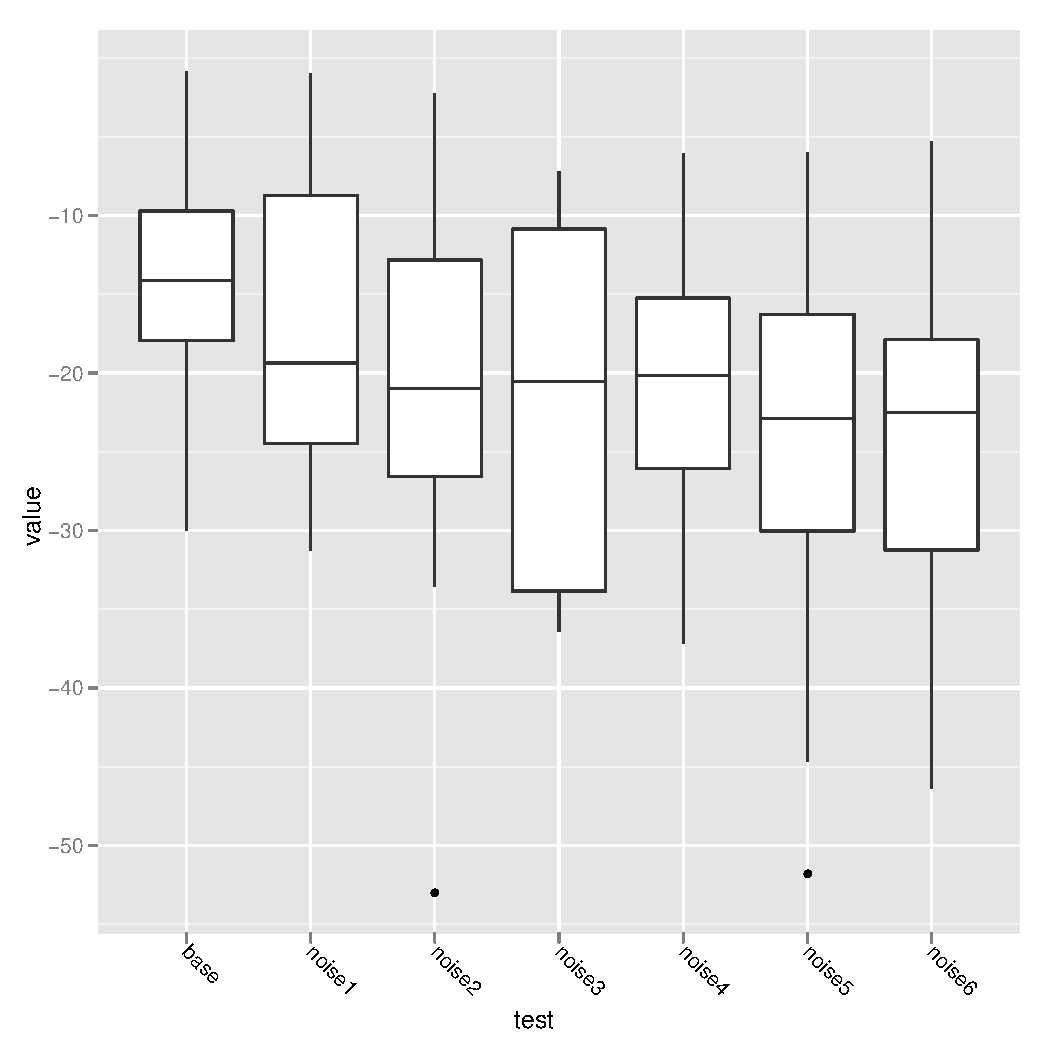
\includegraphics[scale=0.53]{exp/uncert/dtlz1_c10_noise}
      \label{dtlz1_c10_noise}
    }
    \subfloat[DTLZ7 four-criteria]{
      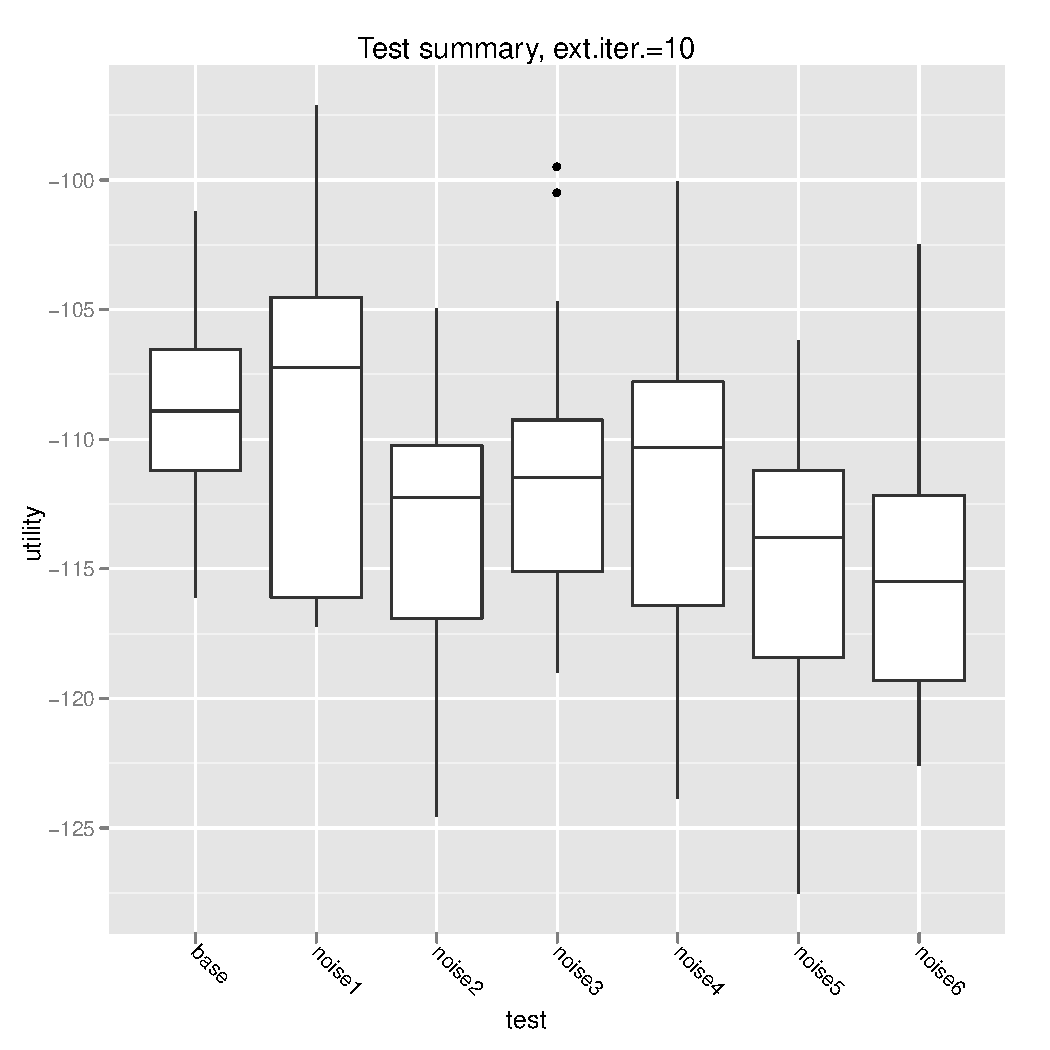
\includegraphics[scale=0.53]{exp/uncert/dtlz7_c4_noise}
      \label{dtlz7_c4_noise}
    }
  }
  \caption{Effect of noise in DM's decisions}
  \label{noise}
\end{figure}


\begin{table}[htb]
  \centering
  \begin{tabular}{r c c c c c c}
    & \multicolumn{3}{c}{Mix problem} & \multicolumn{3}{c}{DTLZ1 c4} \\
    \hline
    noise level & mean & sd & improvement & mean & sd & improvement \\
    \hline
    \hline
    base & 6678.95 & 53.86 & 0.00\% & -12.81 & 8.38 & 0.00\% \\
    noise1 & 6662.93 & 36.54 & -0.24\% & -7.70 & 8.48 & 39.89\% \\
    noise2 & 6638.77 & 70.33 & -0.60\% & -12.61 & 11.36 & 1.55\% \\
    noise3 & 6636.90 & 53.88 & -0.63\% & -12.73 & 10.82 & 0.61\% \\
    noise4 & 6537.39 & 137.71 & -2.12\% & -13.65 & 7.84 & -6.55\% \\
    noise5 & 6093.31 & 811.58 & -8.77\% & -17.27 & 11.32 & -34.82\% \\
    noise6 & 5858.94 & 924.72 & -12.28\% & -13.72 & 12.45 & -7.09\% \\
    \hline
  \end{tabular}
  \caption{The impact of noise in robust environment}
  \label{t:un_noise_1}
\end{table}

 \begin{table}[htb]
  \centering
  \begin{tabular}{r c c c c c c}
    & \multicolumn{3}{c}{DTLZ1 c10} & \multicolumn{3}{c}{DTLZ7 c4} \\
    \hline
    noise level & mean & sd & improvement & mean & sd & improvement \\
    \hline
    \hline
    base & -13.73 & 8.08 & 0.00\% & -108.86 & 4.00 & 0.00\% \\
    noise1 & -17.34 & 9.07 & -26.23\% & -109.48 & 7.03 & -0.57\% \\
    noise2 & -20.58 & 13.18 & -49.83\% & -115.45 & 7.33 & -6.06\% \\
    noise3 & -21.52 & 11.72 & -56.70\% & -112.61 & 5.84 & -3.45\% \\
    noise4 & -21.47 & 9.29 & -56.36\% & -112.38 & 6.51 & -3.24\% \\
    noise5 & -24.86 & 13.03 & -81.01\% & -117.84 & 6.78 & -8.26\% \\
    noise6 & -24.89 & 11.79 & -81.21\% & -117.45 & 7.21 & -7.89\% \\
    \hline
  \end{tabular}
  \caption{The impact of noise in robust environment}
  \label{t:un_noise_2}
\end{table}

\clearpage{}
\subsection{DomLem parameters}

\begin{table}[htb]
  \centering
  \begin{tabular}{r c c c c c c c}
    & & \multicolumn{3}{c}{Mix problem} & \multicolumn{3}{c}{DTLZ1 c4} \\
    \hline
    test & good count & mean & sd & improvement & mean & sd & improvement \\
    \hline
    \hline
domlem             & 3   & 6676.25 & 50.34 & 0.00\% & -16.45 & 13.80 & 0.00\% \\
domlem             & 15 & 6649.69 & 37.74 & -0.40\% & -19.51 & 10.97 & -18.59\% \\
domlem conf 0.6 & 3   & 6655.11 & 43.51 & -0.32\% & -17.44 & 9.48 & -5.99\% \\
domlem conf 0.6 & 15 & 6695.45 & 59.81 & 0.29\% & -19.06 & 15.29 & -15.87\% \\
domlem conf 0.8 & 3   &  6662.44 & 56.97 & -0.21\% & -20.61 & 16.91 & -25.27\% \\
domlem conf 0.8 & 15 & 6662.55 & 66.35 & -0.21\% & -10.28 & 7.88 & \textbf{37.52\%} \\
domlem multirules & 3  & 6680.08 & 33.44 & 0.06\% & -6.74 & 5.60 & \textbf{59.00\%} \\
domlem multirules & 15 & 6658.61 & 27.97 & -0.26\% & -12.83 & 10.38 & \textbf{22.00\%} \\    \hline
  \end{tabular}
  \caption{Influence of the DomLem parameters in robust environment}
  \label{t:un_domlem_1}
\end{table}

 \begin{table}[htb]
  \centering
  \begin{tabular}{r c c c c c c c}
    & & \multicolumn{3}{c}{DTLZ1 c10} & \multicolumn{3}{c}{DTLZ7 c4} \\
    \hline
    test & good count & mean & sd & improvement & mean & sd & improvement \\
    \hline
    \hline
domlem               & 3 & -21.05 & 17.52 & 0.00\% & -108.94 & 4.01 & 0.00\% \\
domlem               & 15 & -15.50 & 9.28 & \textbf{26.35\%} & -109.28 & 4.96 & -0.31\% \\
domlem conf 0.6 & 3 &  -22.44 & 8.82 & -6.60\% & -112.68 & 4.15 & -3.43\% \\
domlem conf 0.6 & 15 & -9.09 & 7.39 & \textbf{56.82\%} & -109.28 & 7.95 & -0.31\% \\
domlem conf 0.8 & 3 &  -22.66 & 14.83 & -7.67\% & -108.83 & 5.28 & 0.10\% \\
domlem conf 0.8 &  15 &-26.76 & 17.14 & -27.14\% & -108.53 & 7.29 & 0.38\% \\
domlem multirules & 3 &  -18.14 & 14.80 & 13.81\% & -112.03 & 5.79 & -2.83\% \\
domlem multirules &  15 &-17.71 & 10.34 & 15.86\% & -110.17 & 5.48 & -1.13\% \\
    \hline
  \end{tabular}
  \caption{Influence of the DomLem parameters in robust environment}
  \label{t:un_domlem_2}
\end{table}


\begin{figure}
  \centering
  \makebox[\textwidth]{
    \subfloat{
      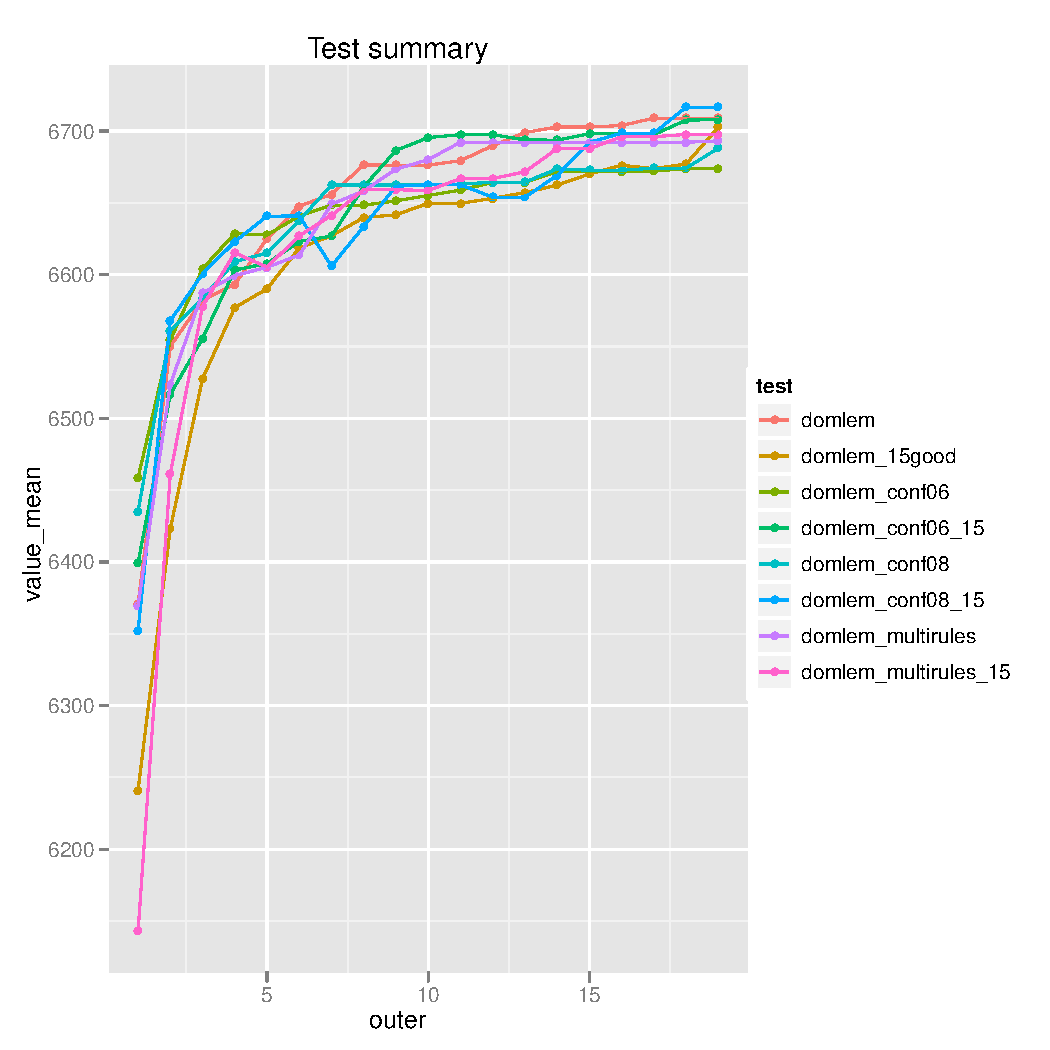
\includegraphics[scale=0.53]{exp/uncert/algo_dom/presentation}
      \label{pres_domlem1}
    }
    \subfloat{
      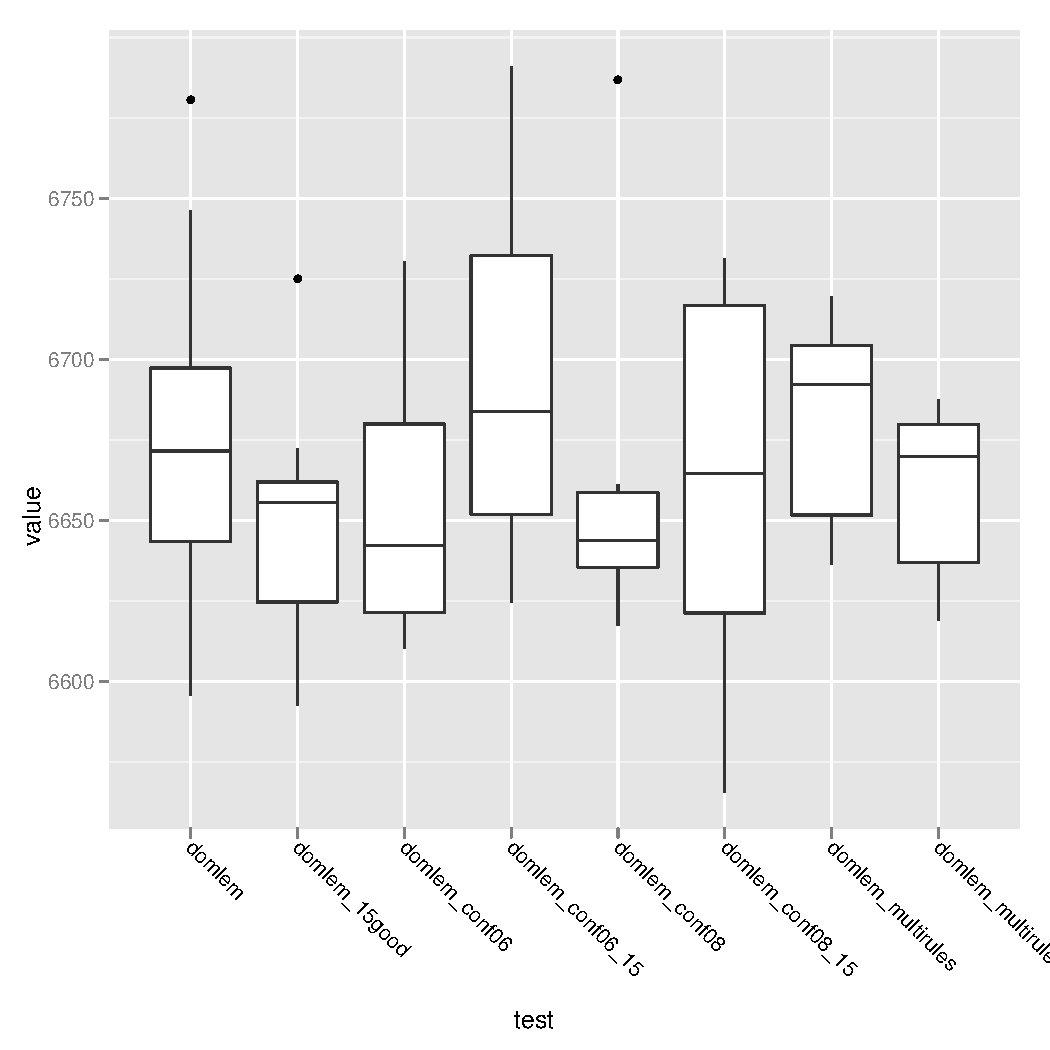
\includegraphics[scale=0.53]{exp/uncert/algo_dom/presentationb}
      \label{pres_domlem1b}
    }
  }
  \caption{Influence of the DomLem parameters on the mix problem}
  \label{pres_domlem}
\end{figure}

\begin{figure}
  \centering
  \makebox[\textwidth]{
    \subfloat{
      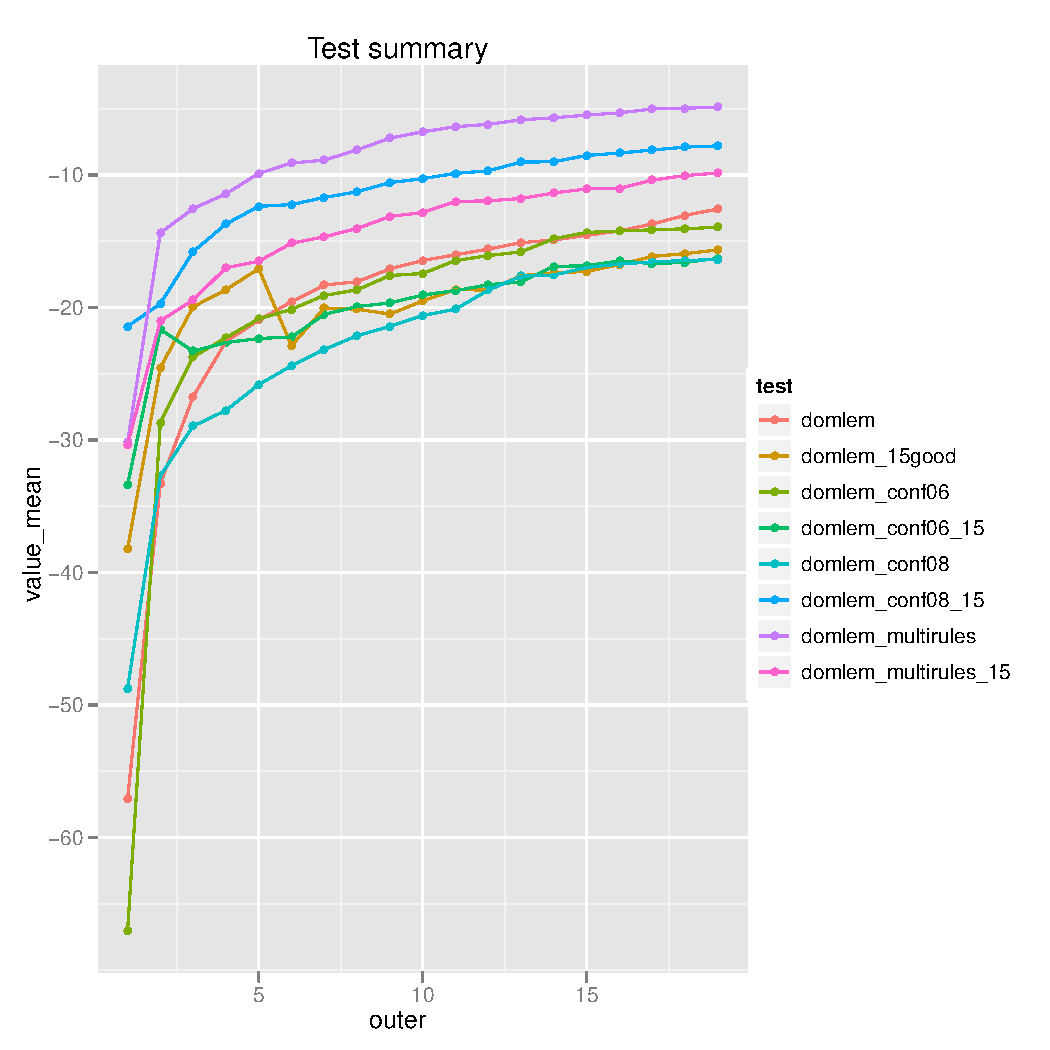
\includegraphics[scale=0.53]{exp/uncert/algo_dom/dtlz1_c4}
      \label{dtlz1_c4_domlem1}
    }
    \subfloat{
      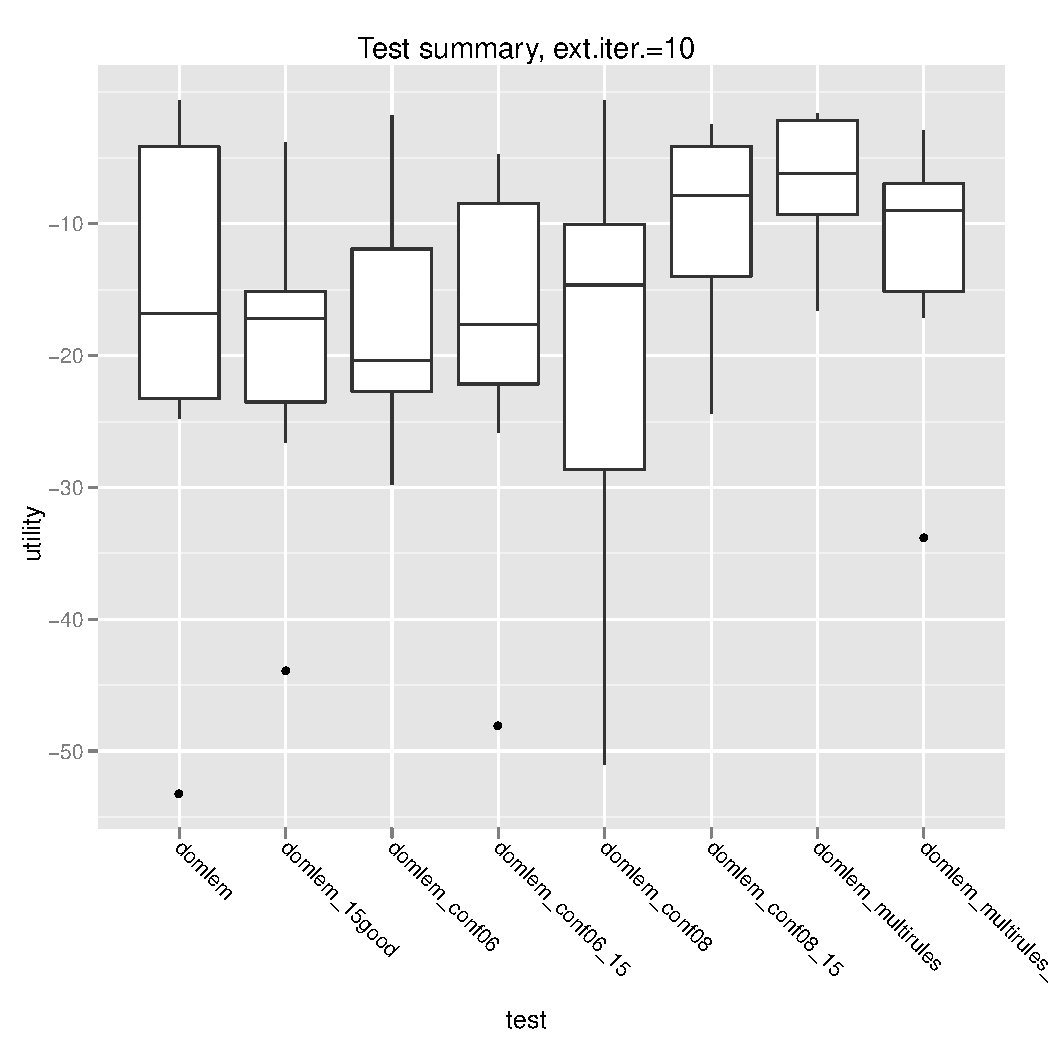
\includegraphics[scale=0.53]{exp/uncert/algo_dom/dtlz1_c4b}
      \label{dtlz1_c4_domlem1b}
    }
  }
  \caption{Influence of the DomLem parameters on the four-criteria DTLZ1 problem}
  \label{dtlz1_c4_domlem}
\end{figure}

\begin{figure}
  \centering
  \makebox[\textwidth]{
    \subfloat{
      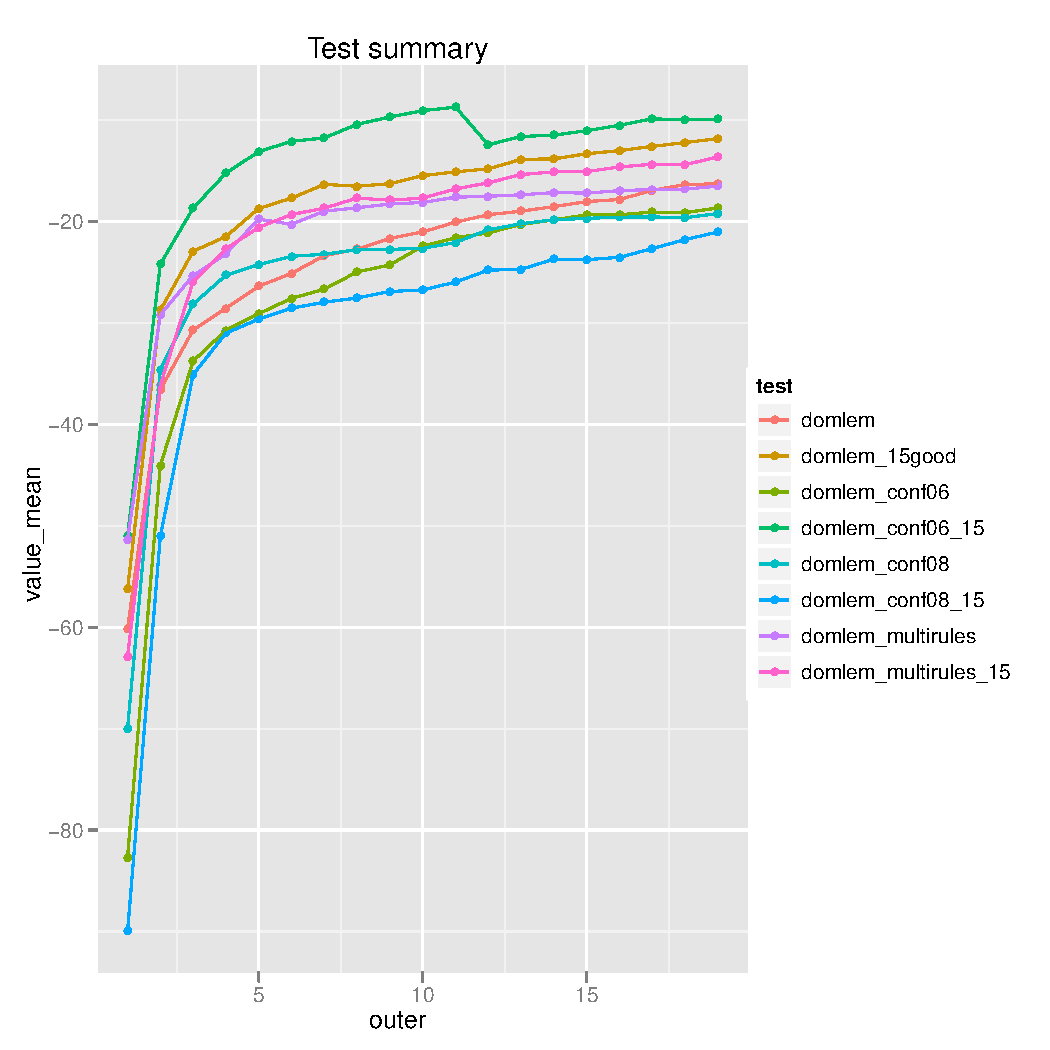
\includegraphics[scale=0.53]{exp/uncert/algo_dom/dtlz1_c10}
      \label{dtlz1_c10_domlem1}
    }
    \subfloat{
      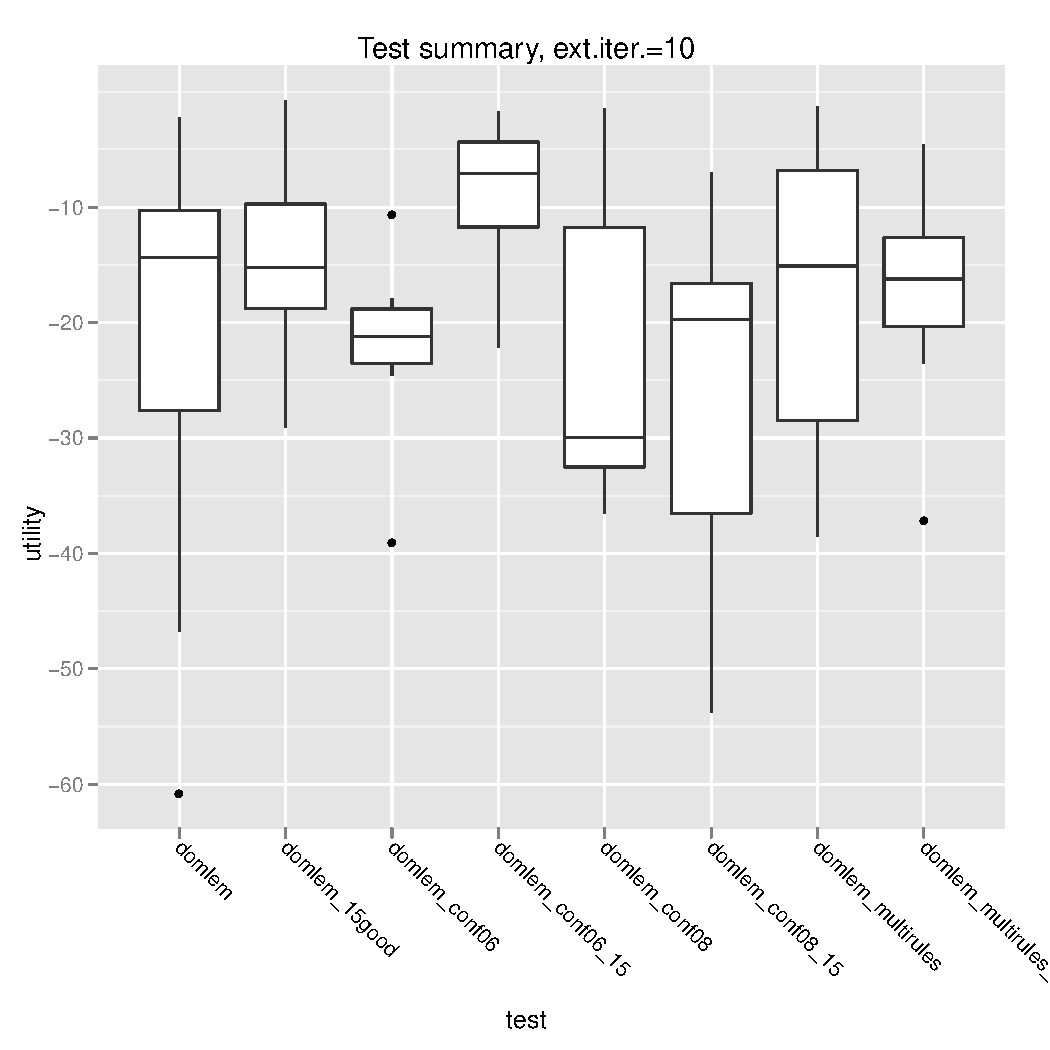
\includegraphics[scale=0.53]{exp/uncert/algo_dom/dtlz1_c10b}
      \label{dtlz1_c10_domlem1b}
    }
  }
  \caption{Influence of the DomLem parameters on the ten-criteria DTLZ1 problem}
  \label{dtlz1_c10_domlem}
\end{figure}

\begin{figure}
  \centering
  \makebox[\textwidth]{
    \subfloat{
      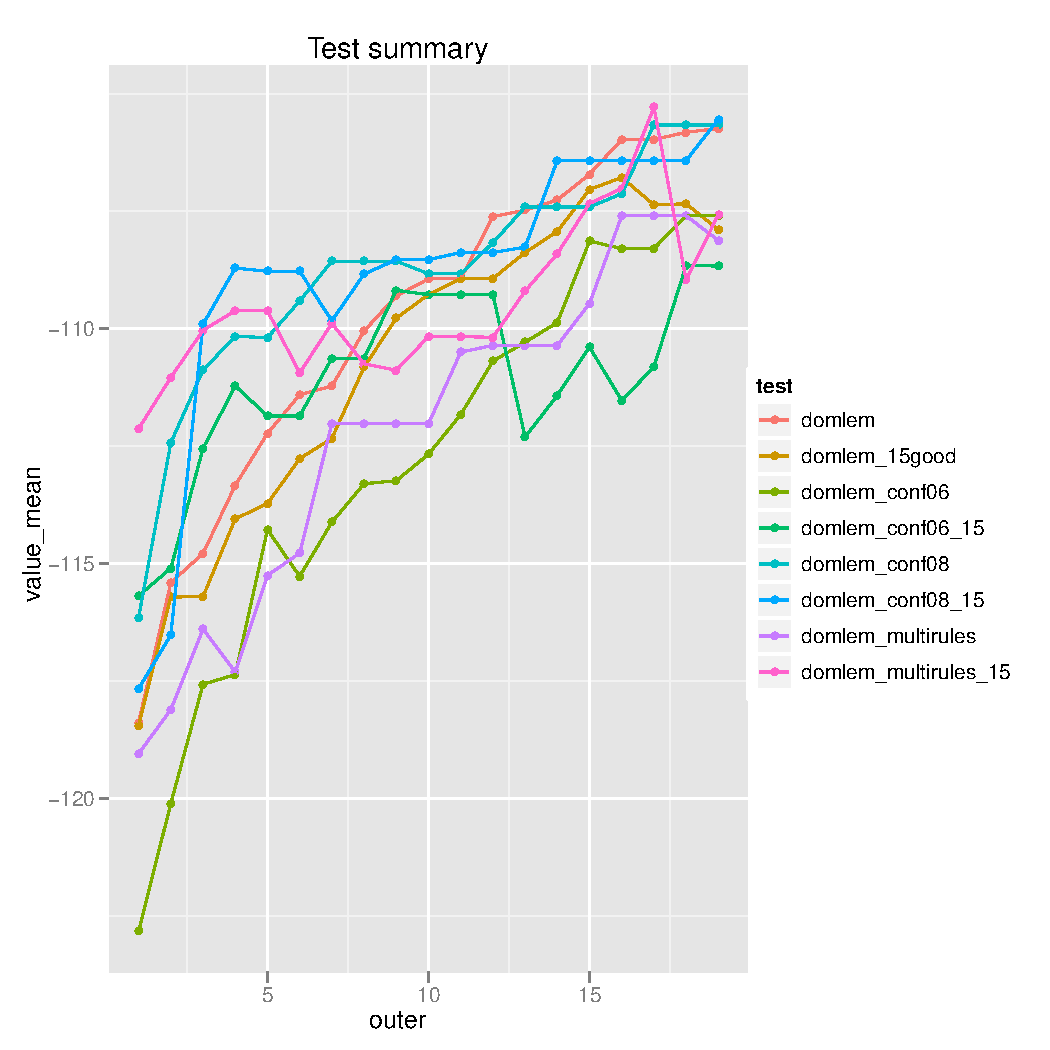
\includegraphics[scale=0.53]{exp/uncert/algo_dom/dtlz7_c4}
      \label{dtlz7_c4_domlem1}
    }
    \subfloat{
      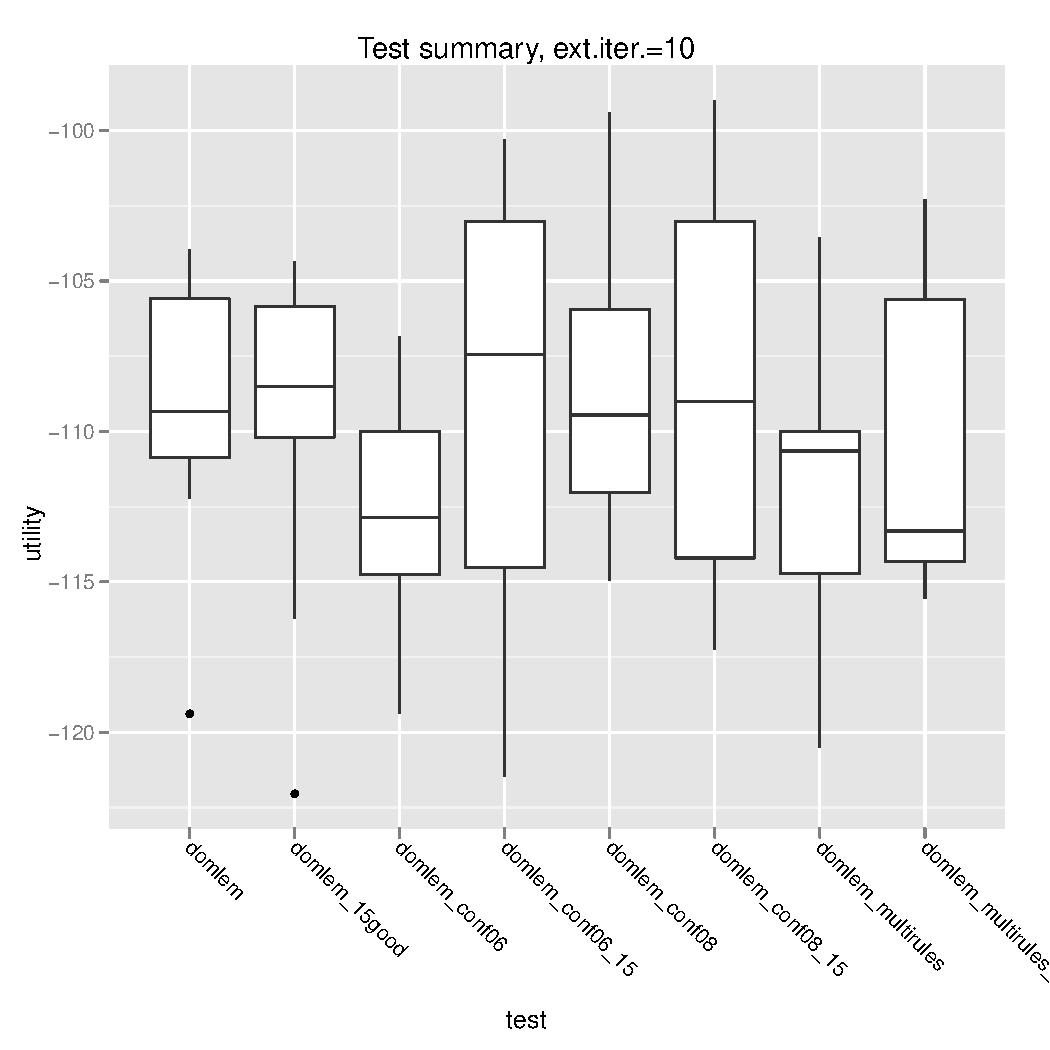
\includegraphics[scale=0.53]{exp/uncert/algo_dom/dtlz7_c4b}
      \label{dtlz7_c4_domlem1b}
    }
  }
  \caption{Performance comparison on the four-criteria DTLZ7 problem}
  \label{dtlz7_c4_perf}
\end{figure}


\clearpage{}
\subsection{AllRules algorithm}

\begin{table}[htb]
  \centering
  \begin{tabular}{r c c c c c c c}
    & & \multicolumn{3}{c}{Mix problem} & \multicolumn{3}{c}{DTLZ1 c4} \\
    \hline
    test & good count & mean & sd & improvement & mean & sd & improvement \\
    \hline
    \hline
allrules & 3 & 6658.39 & 69.98 & 0.00\% & -13.05 & 11.80 & 0.00\% \\
allrules & 15& 6572.14 & 79.91 & -1.30\% & -4.52 & 3.05 & 65.36\% \\
\hline
  \end{tabular}
  \caption{AllRules --- number of solutions chosen and its influence on the result}
  \label{t:un_allrules_1}
\end{table}

 \begin{table}[htb]
  \centering
  \begin{tabular}{r c c c c}
    & & \multicolumn{3}{c}{DTLZ7 c4} \\
    \hline
    test & good count & mean & sd & improvement \\
    \hline
    \hline
allrules & 3 &-111.80 & 3.68 & 0.00\% \\
allrules &15 & -110.07 & 7.84 & 1.55\% \\
    \hline
  \end{tabular}
  \caption{AllRules --- number of solutions chosen and its influence on the result}
  \label{t:un_allrules_2}
\end{table}


\begin{table}[htb]
  \centering
  \begin{tabular}{l l c c c c}
    \hline
    problem & test & good count & mean & sd & improvement \\
    \hline
    \hline
mix problem & allrules & 3 & 6658.39 & 69.98 & 0.00\% \\
mix problem & domlem conf 0.6 & 15 & 6695.45 & 59.81 &\textbf{ 0.56\%} \\
\hline
dtlz1 four criteria & allrules & 15 & -4.52 & 3.05 & \textbf{0.00\%} \\
dtlz1 four criteria & domlem & 3 & -16.45 & 13.80 & -263.83\% \\
\hline
dtlz7 four criteria & allrules & 15 & -110.07 & 7.84 & 0.00\% \\
dtlz7 four criteria & domlem conf 0.8 & 15 & -108.53 & 7.29 & \textbf{1.40\%} \\
    \hline
  \end{tabular}
  \caption{AllRules and DomLem comparison}
  \label{t:un_alldom_2}
\end{table}



\begin{figure}
  \centering
  \makebox[\textwidth]{
    \subfloat{
      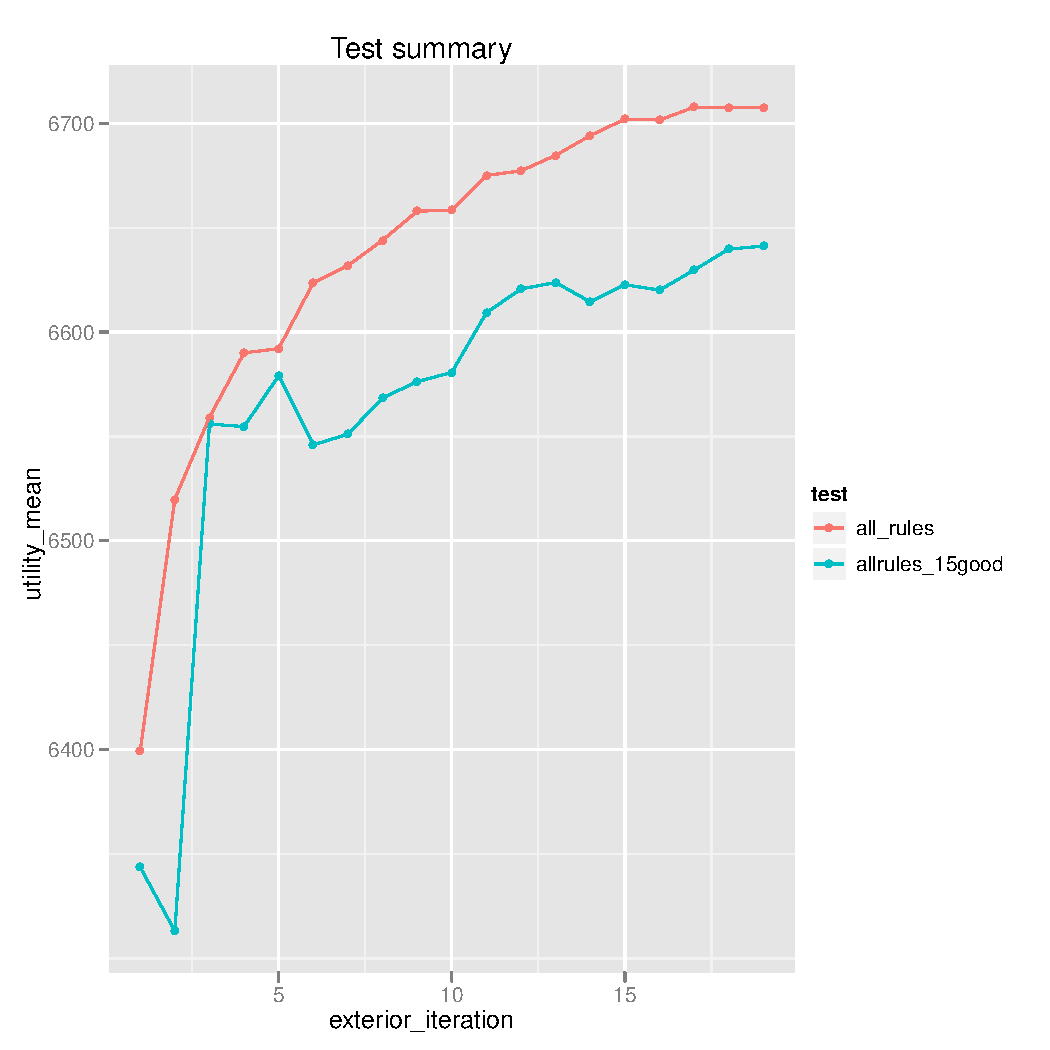
\includegraphics[scale=0.53]{exp/uncert/algo_all/presentation}
      \label{pres_allrules1}
    }
    \subfloat{
      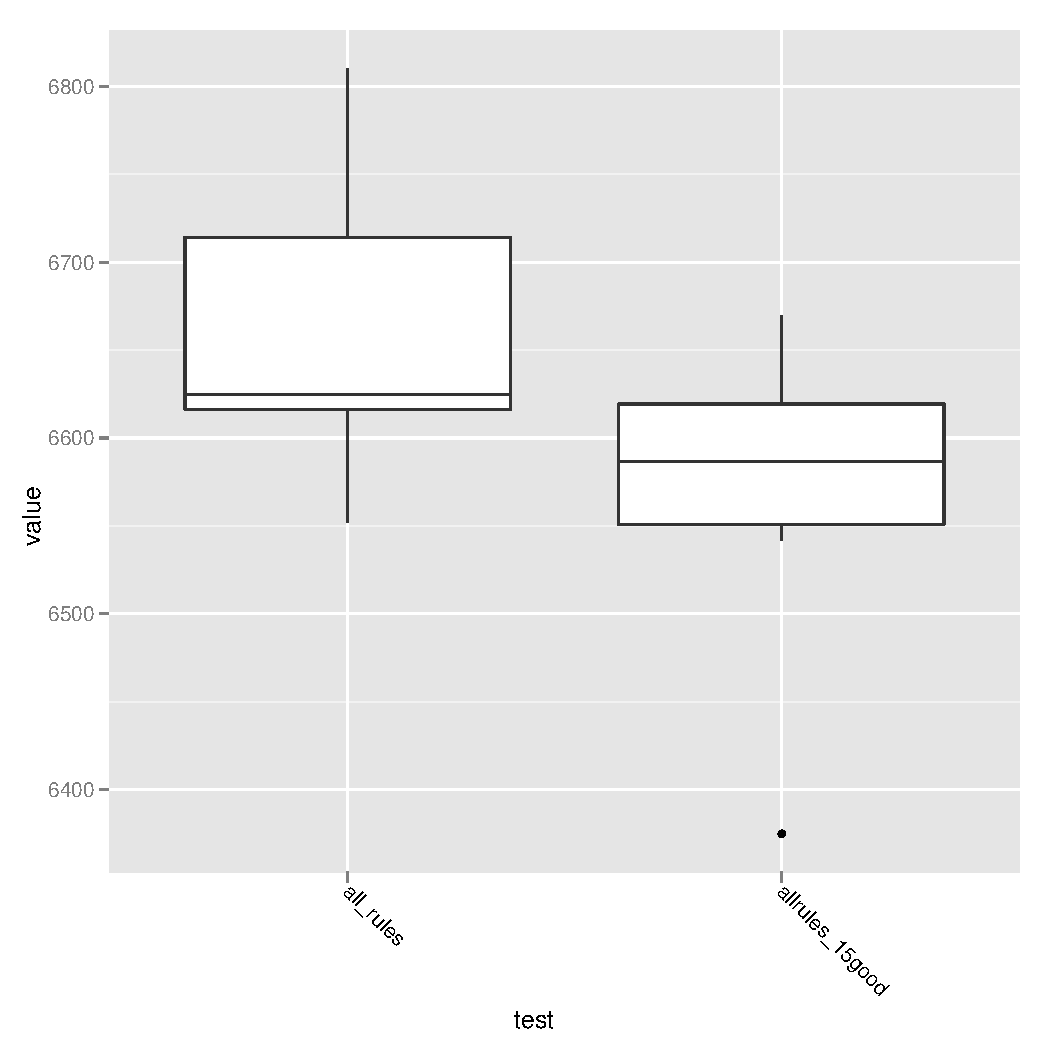
\includegraphics[scale=0.53]{exp/uncert/algo_all/presentationb}
      \label{pres_allrules1b}
    }
  }
  \caption{AllRules --- number of solutions chosen and its influence on the mix problem}
  \label{pres_allrules}
\end{figure}

\begin{figure}
  \centering
  \makebox[\textwidth]{
    \subfloat{
      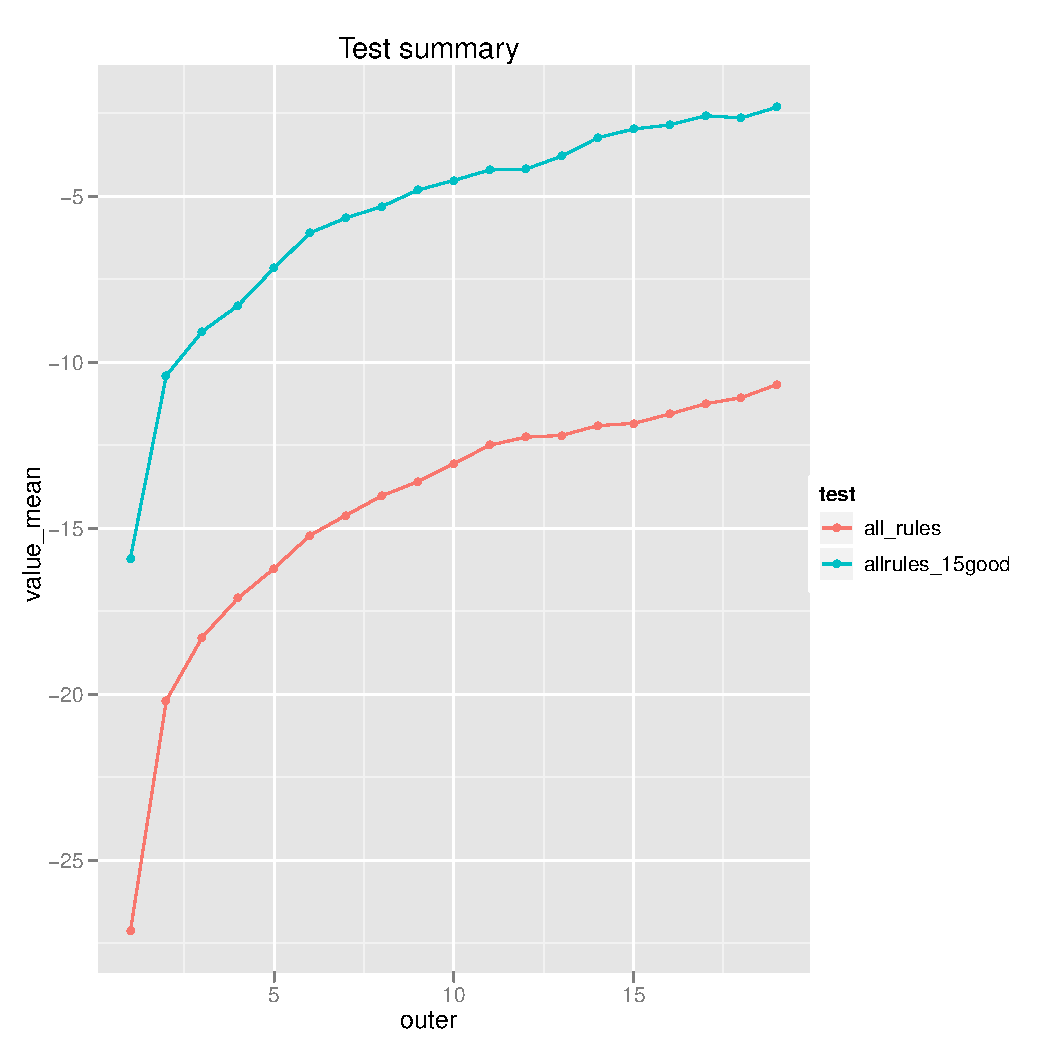
\includegraphics[scale=0.53]{exp/uncert/algo_all/dtlz1_c4}
      \label{dtlz1_c4_allrules1}
    }
    \subfloat{
      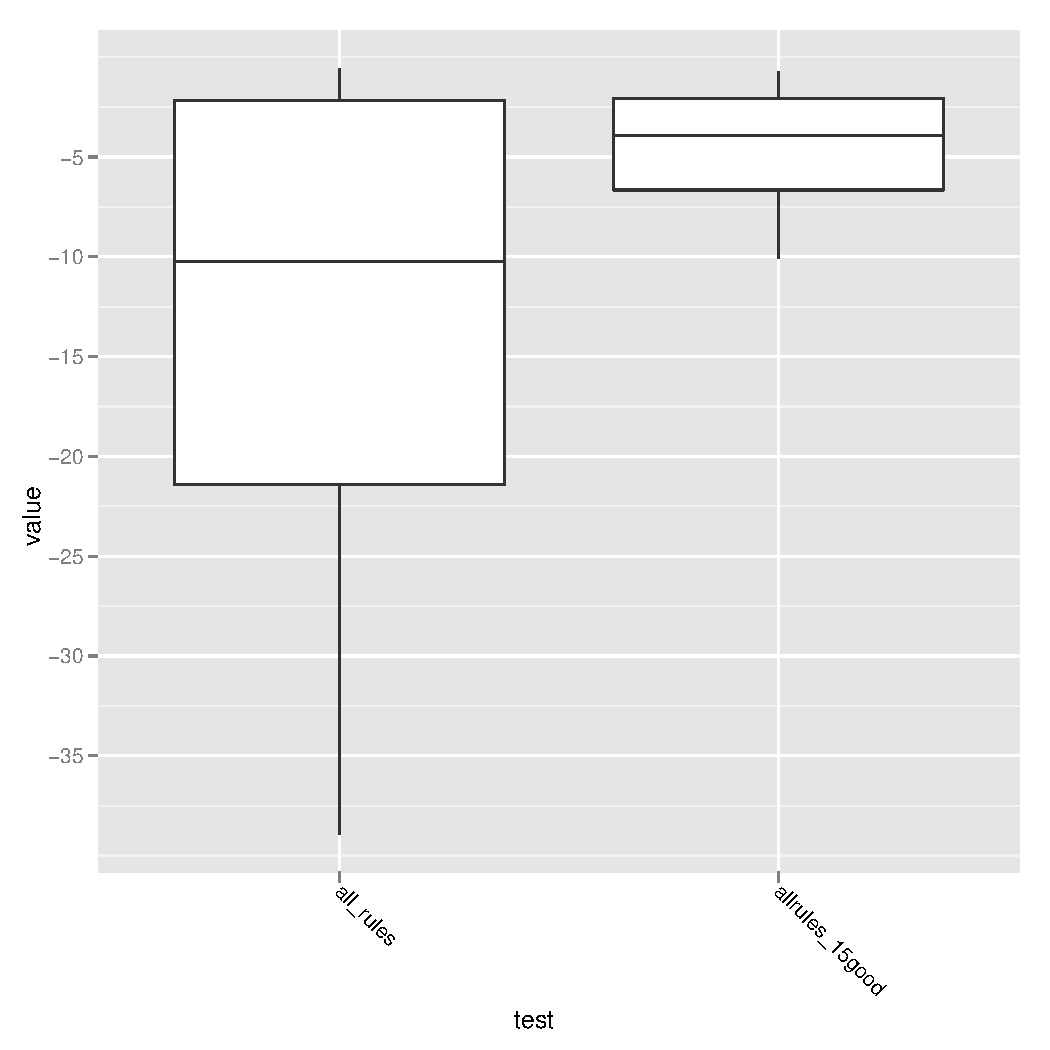
\includegraphics[scale=0.53]{exp/uncert/algo_all/dtlz1_c4b}
      \label{dtlz1_c4_allrules1b}
    }
  }
  \caption{AllRules --- number of solutions chosen and its influence on the four-criteria DTLZ1 problem}
  \label{dtlz1_c4_allrules}
\end{figure}

\begin{figure}
  \centering
  \makebox[\textwidth]{
    \subfloat{
      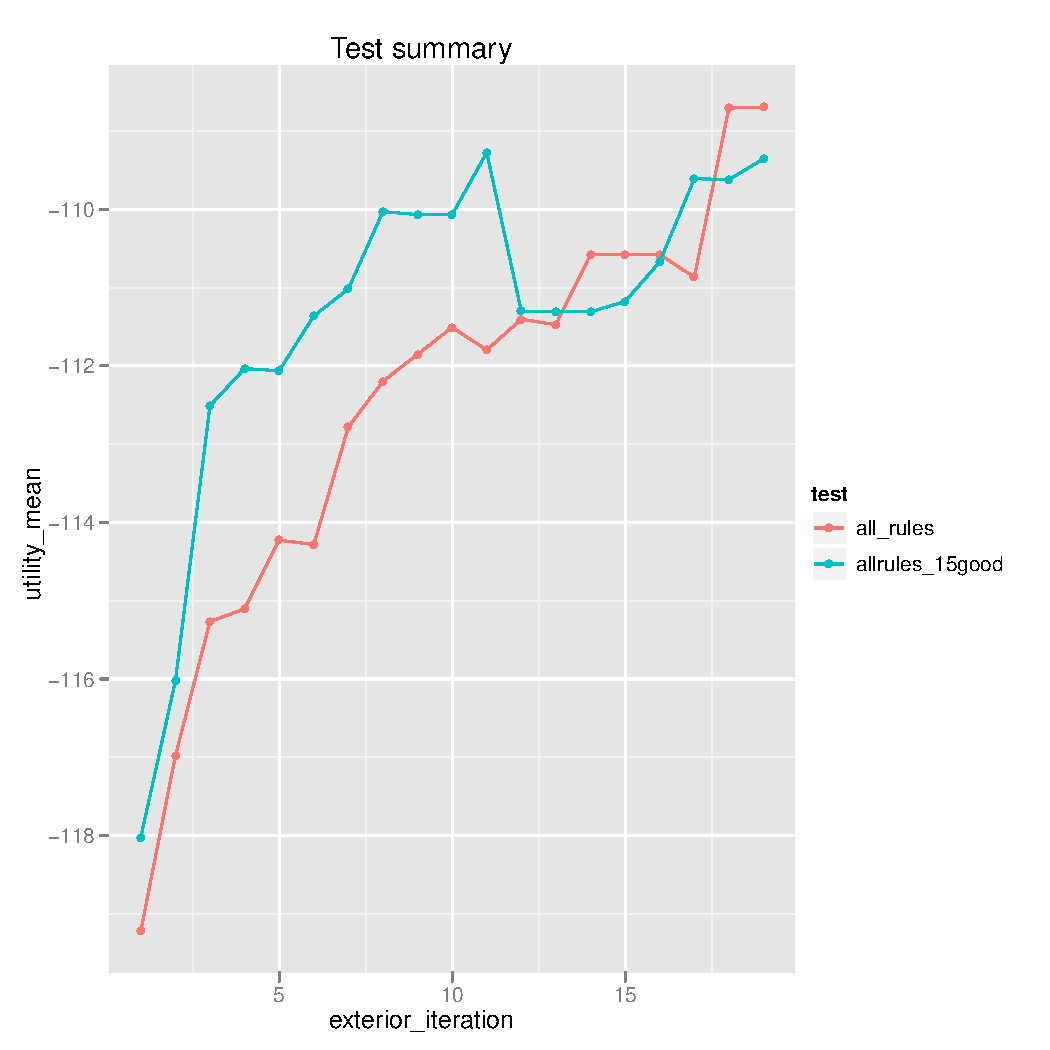
\includegraphics[scale=0.53]{exp/uncert/algo_all/dtlz7_c4}
      \label{dtlz7_c4_allrules}
    }
    \subfloat{
      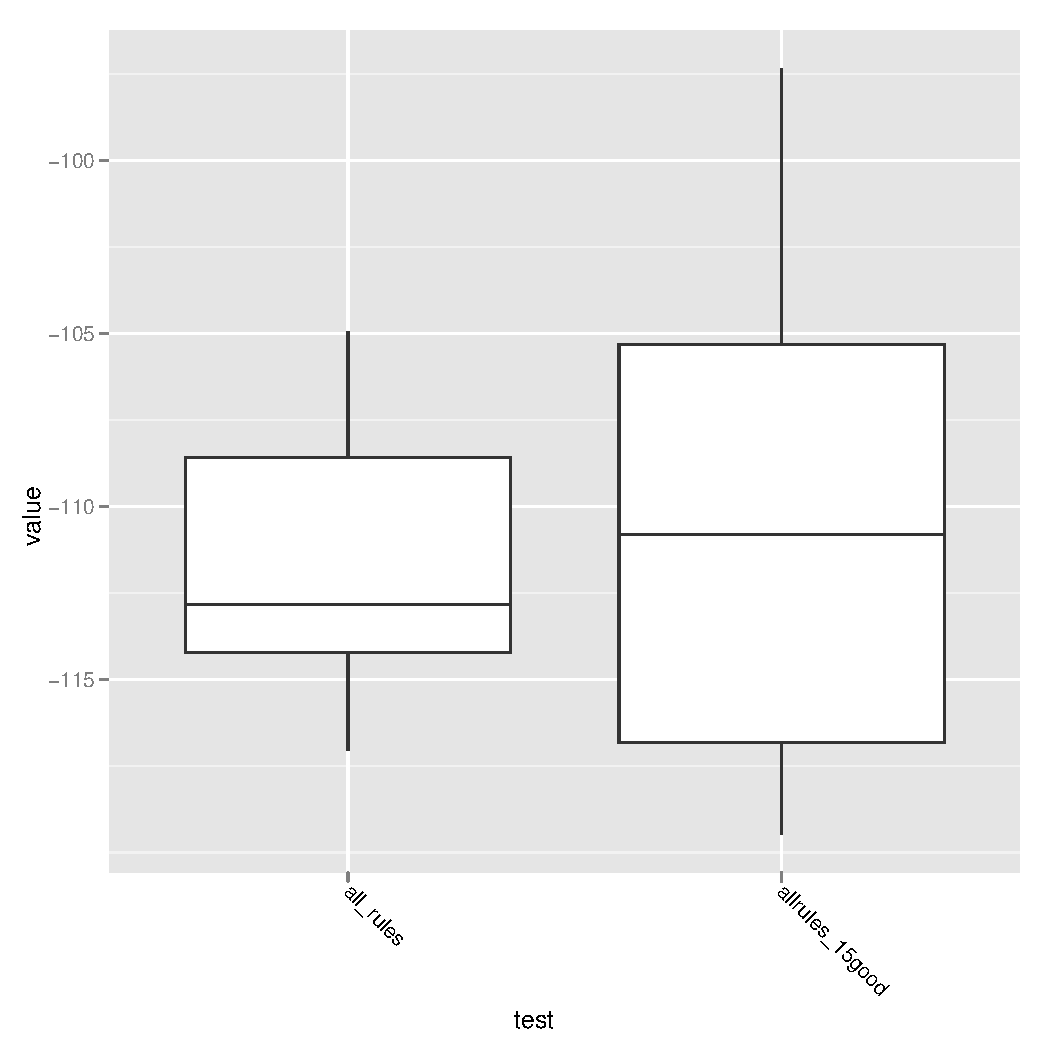
\includegraphics[scale=0.53]{exp/uncert/algo_all/dtlz7_c4b}
      \label{dtlz7_c4_allrules}
    }
  }
  \caption{AllRules --- number of solutions chosen and its influence on the four-criteria DTLZ7 problem}
  \label{dtlz7_c4_allrules}
\end{figure}


\begin{figure}
  \centering
  \makebox[\textwidth]{
    \subfloat{
      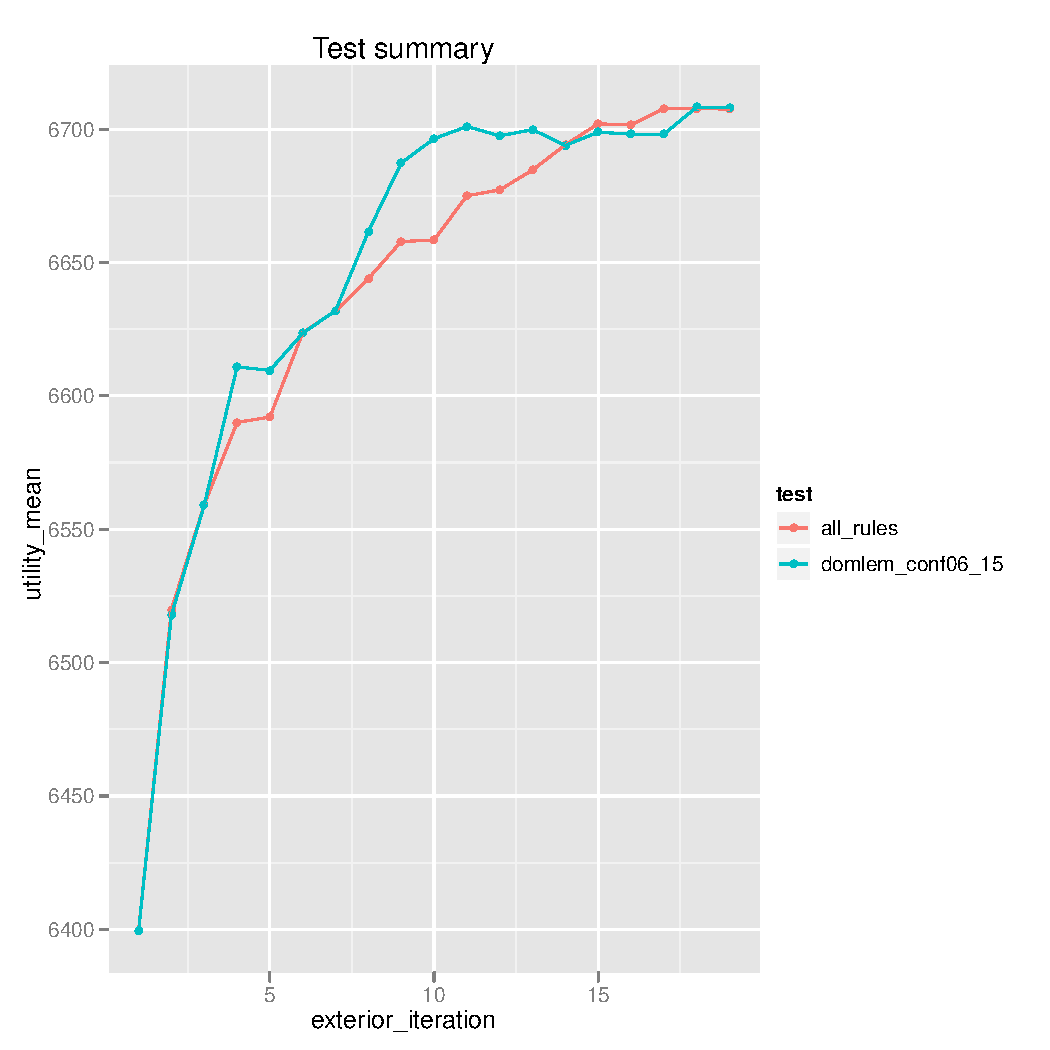
\includegraphics[scale=0.53]{exp/uncert/algo_allvsdom/presentation}
      \label{pres_alldom}
    }
    \subfloat{
      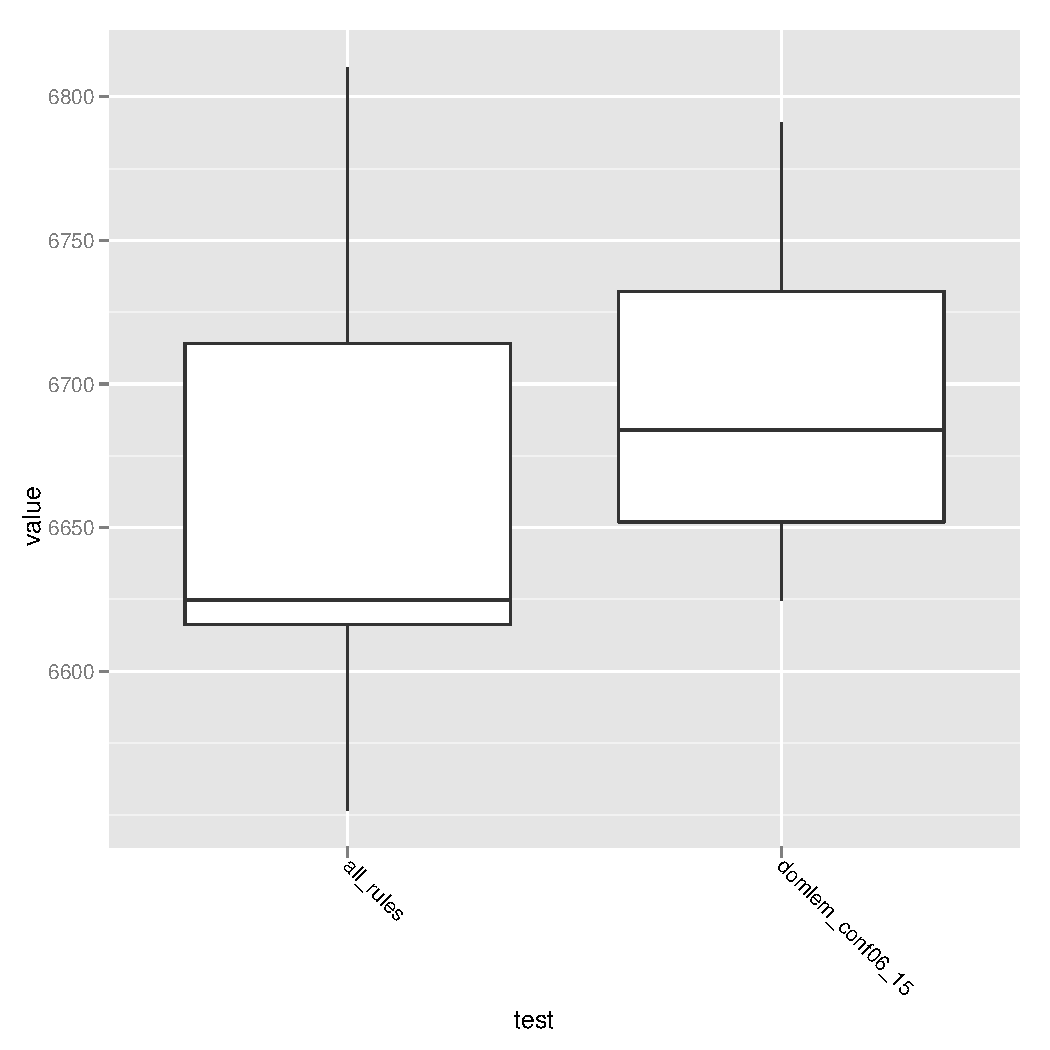
\includegraphics[scale=0.53]{exp/uncert/algo_allvsdom/presentationb}
      \label{pres_alldom}
    }
  }
  \caption{AllRules and DomLem comparison on the mix problem}
  \label{pres_alldom}
\end{figure}

\begin{figure}
  \centering
  \makebox[\textwidth]{
    \subfloat{
      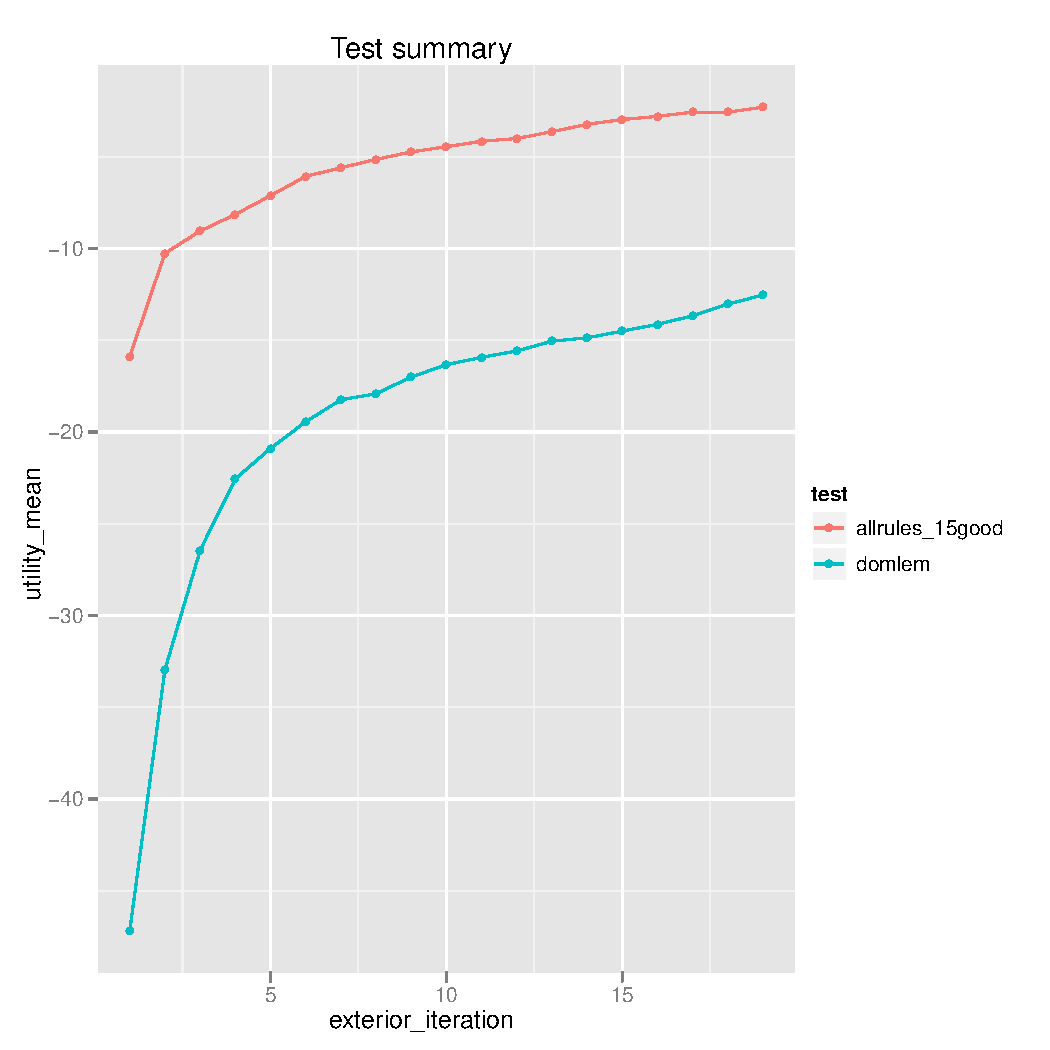
\includegraphics[scale=0.53]{exp/uncert/algo_allvsdom/dtlz1_c4}
      \label{dtlz1_c4_alldom}
    }
    \subfloat{
      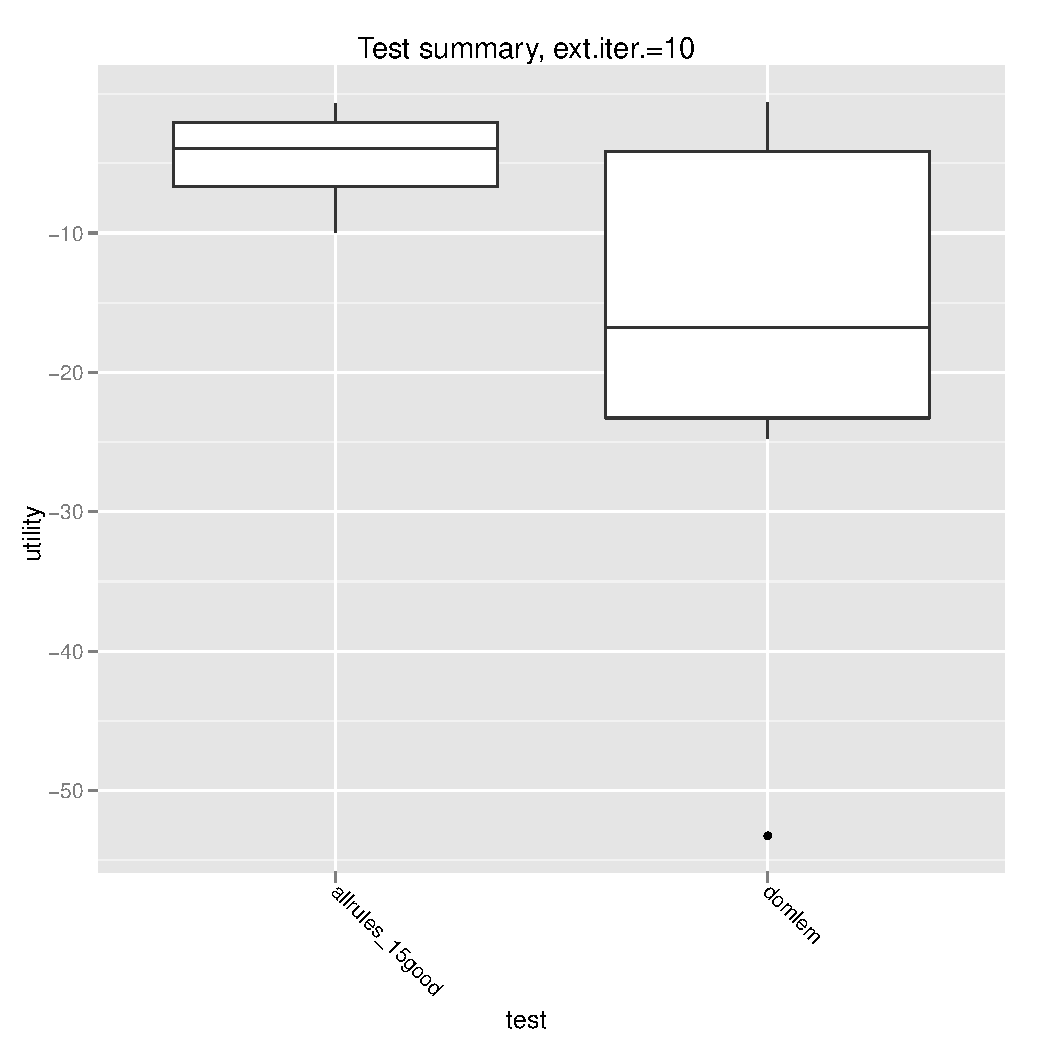
\includegraphics[scale=0.53]{exp/uncert/algo_allvsdom/dtlz1_c4b}
      \label{dtlz1_c4_alldom}
    }
  }
  \caption{AllRules and DomLem comparison on the four-criteria DTLZ1 problem}
  \label{dtlz1_c4_alldom}
\end{figure}

\begin{figure}
  \centering
  \makebox[\textwidth]{
    \subfloat{
      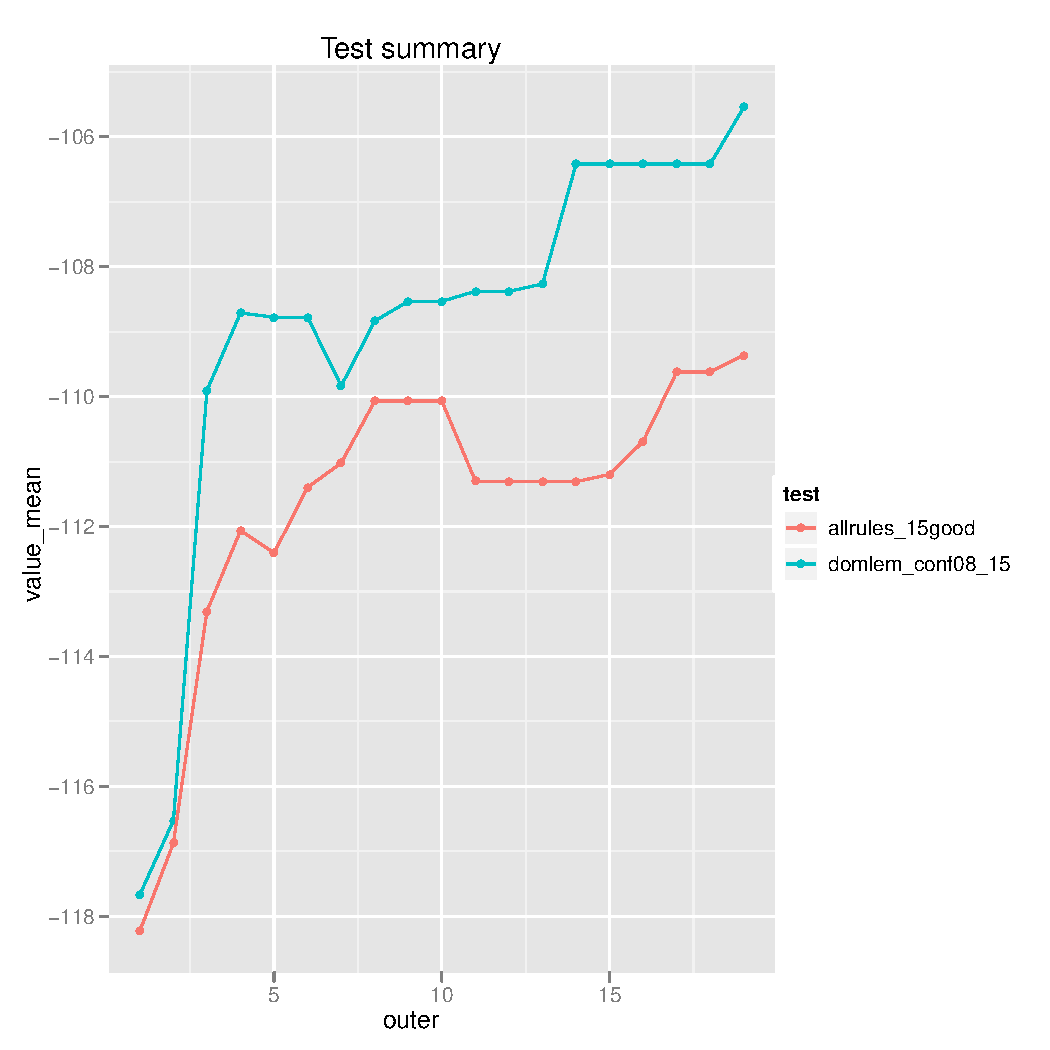
\includegraphics[scale=0.53]{exp/uncert/algo_allvsdom/dtlz7_c4}
      \label{dtlz7_c4_alldom}
    }
    \subfloat{
      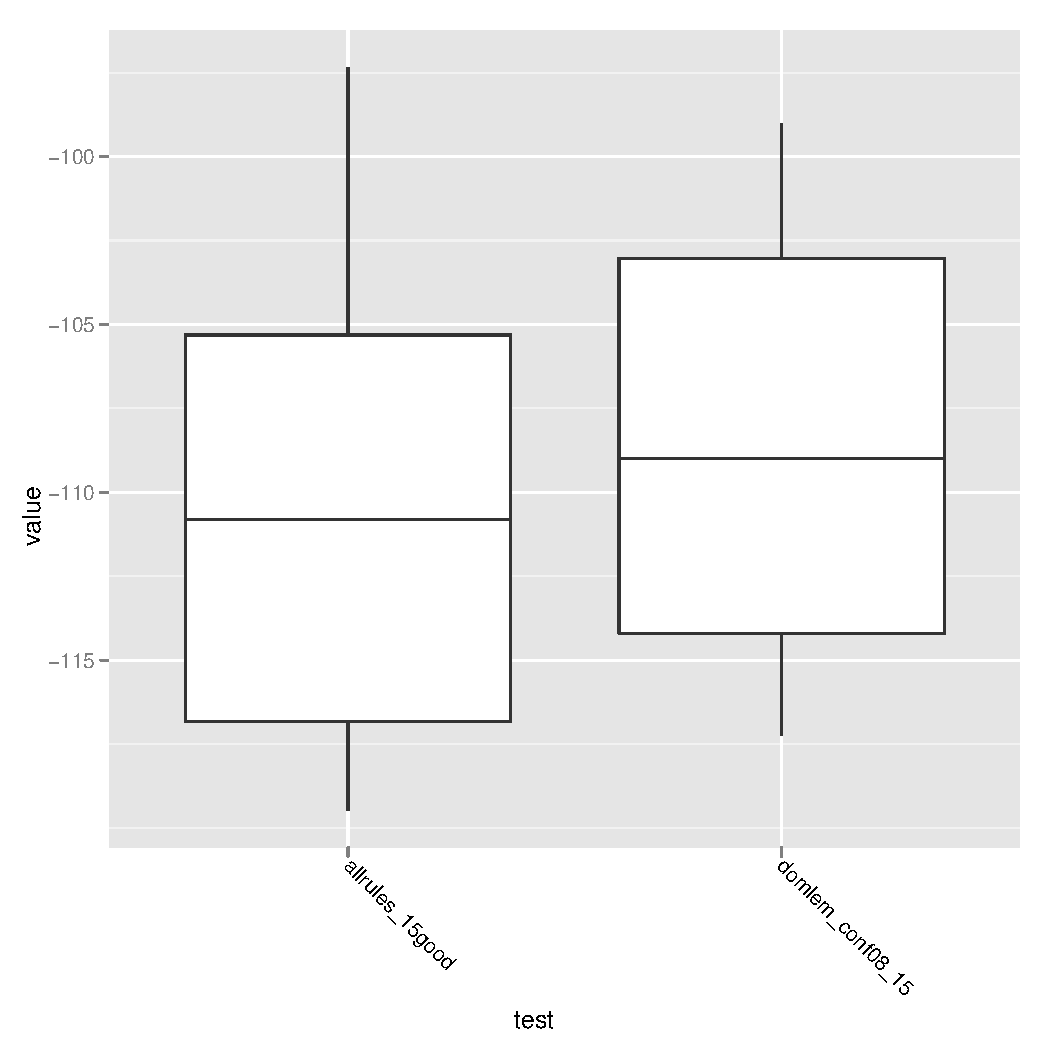
\includegraphics[scale=0.53]{exp/uncert/algo_allvsdom/dtlz7_c4b}
      \label{dtlz7_c4_alldom}
    }
  }
  \caption{AllRules and DomLem comparison on the four-criteria DTLZ7 problem}
  \label{dtlz7_c4_alldom}
\end{figure}


\clearpage{}
\subsection{Average in quantiles}
\textcolor{green}{TODO}



\subsection{Best results}


\begin{table}[htb]
  \centering
  \begin{tabular}{l c c c c c}
    \hline
outer & mean supposed utility & supp stddev & domlem conf 0.6 15 & stddev & improvement \\
    \hline
    \hline
1 & 6551.03 & 105.13 & 6399.34 & 208.67 & -2.32\% \\
2 & 6618.31 & 59.98 & 6516.66 & 108.81 & -1.54\% \\
3 & 6627.03 & 55.99 & 6555.59 & 94.60 & -1.08\% \\
4 & 6641.97 & 56.68 & 6603.19 & 88.61 & -0.58\% \\
5 & 6646.64 & 52.71 & 6607.81 & 90.20 & -0.58\% \\
6 & 6657.24 & 43.55 & 6623.12 & 70.84 & -0.51\% \\
7 & 6660.01 & 42.18 & 6626.90 & 55.62 & -0.50\% \\
8 & 6674.68 & 41.26 & 6661.15 & 78.86 & -0.20\% \\
9 & 6678.98 & 42.18 & 6686.50 & 68.39 & 0.11\% \\
10 & 6678.98 & 42.18 & 6695.45 & 59.81 & 0.25\% \\
11 & 6682.55 & 38.42 & 6697.46 & 54.06 & 0.22\% \\
12 & 6688.63 & 42.88 & 6697.46 & 54.06 & 0.13\% \\
13 & 6688.88 & 42.58 & 6693.87 & 59.44 & 0.07\% \\
14 & 6688.88 & 42.58 & 6693.59 & 59.62 & 0.07\% \\
15 & 6691.59 & 40.16 & 6698.10 & 57.73 & 0.10\% \\
16 & 6695.68 & 41.14 & 6698.10 & 57.73 & 0.04\% \\
17 & 6701.35 & 39.70 & 6697.50 & 57.20 & -0.06\% \\
18 & 6701.35 & 39.70 & 6707.60 & 46.91 & 0.09\% \\
19 & 6710.87 & 40.02 & 6707.98 & 47.62 & -0.04\% \\
    \hline
  \end{tabular}
  \caption{Best run for the mix problem}
  \label{t:un_best_1}
\end{table}


\begin{table}[htb]
  \centering
  \begin{tabular}{l c c c c c}
    \hline
outer & mean supposed utility & supp stddev & allrules 15 & stddev & improvement \\
    \hline
    \hline
1 & -18.3391432 & 9.816309925 & -15.9057201 & 5.855560357 & 13.27\% \\
2 & -13.2356894 & 8.624514343 & -10.3998425 & 4.765240651 & 21.43\% \\
3 & -11.94097973 & 8.741655213 & -9.0707026 & 4.40860178 & 24.04\% \\
4 & -10.79149427 & 8.534598525 & -8.2907986 & 3.942180864 & 23.17\% \\
5 & -9.858469467 & 8.329327334 & -7.1591062 & 3.293595183 & 27.38\% \\
6 & -9.5595594 & 8.4703238 & -6.1006858 & 2.989990226 & 36.18\% \\
7 & -9.245239733 & 8.552617493 & -5.6530246 & 3.231994959 & 38.85\% \\
8 & -8.828774867 & 8.490932909 & -5.3074947 & 3.472475913 & 39.88\% \\
9 & -8.744311933 & 8.500549926 & -4.812787 & 3.265940892 & 44.96\% \\
10 & -8.233213133 & 8.381281926 & -4.5213741 & 3.047627164 & 45.08\% \\
11 & -8.117539467 & 8.375530506 & -4.2083127 & 3.189215908 & 48.16\% \\
12 & -7.759438 & 8.320247724 & -4.1838711 & 3.471391475 & 46.08\% \\
13 & -7.624005867 & 8.403986271 & -3.7924346 & 3.647954718 & 50.26\% \\
14 & -7.305845067 & 8.416626846 & -3.2418574 & 3.552557886 & 55.63\% \\
15 & -7.131843267 & 8.260038646 & -2.9737998 & 3.51227313 & 58.30\% \\
16 & -7.023623867 & 8.200634129 & -2.8526141 & 3.493516972 & 59.39\% \\
17 & -6.884764333 & 8.090375153 & -2.5747586 & 3.35765165 & 62.60\% \\
18 & -6.8254398 & 8.119784484 & -2.6394718 & 3.451976393 & 61.33\% \\
19 & -6.7802564 & 8.09374618 & -2.3148267 & 3.139534874 & 65.86\% \\
    \hline
  \end{tabular}
  \caption{Best run for the four criteria DTLZ1}
  \label{t:un_best_2}
\end{table}


\begin{table}[htb]
  \centering
  \begin{tabular}{l c c c c c}
    \hline
outer & mean supposed utility & supp stddev & domlem conf 0.6 15 & stddev & improvement \\
    \hline
    \hline
1 & -22.0671162 & 11.81221109 & -50.98594943 & 24.75871578 & -131.05\% \\
2 & -15.2574986 & 9.239740188 & -24.21716357 & 16.77122463 & -58.72\% \\
3 & -13.29195727 & 8.487948732 & -18.69859471 & 13.77507211 & -40.68\% \\
4 & -12.0341928 & 8.079224415 & -15.25463729 & 10.52913999 & -26.76\% \\
5 & -11.40818833 & 8.04300494 & -13.12703 & 7.687244559 & -15.07\% \\
6 & -10.60111927 & 7.642058813 & -12.10850086 & 7.460299736 & -14.22\% \\
7 & -10.18095873 & 7.69139632 & -11.78263214 & 7.960205031 & -15.73\% \\
8 & -10.01096693 & 7.772909933 & -10.437213 & 8.285092823 & -4.26\% \\
9 & -9.781664733 & 7.707954471 & -9.715185 & 7.362741762 & 0.68\% \\
10 & -9.5584798 & 7.654400128 & -9.088617143 & 7.392192847 & 4.92\% \\
11 & -9.139964 & 7.736231986 & -8.743928714 & 7.470572912 & 4.33\% \\
12 & -9.002532867 & 7.765302614 & -12.46026357 & 11.1796289 & -38.41\% \\
13 & -8.689782067 & 7.68784697 & -11.63526557 & 10.83305606 & -33.90\% \\
14 & -8.561289733 & 7.66531129 & -11.50929814 & 10.90953999 & -34.43\% \\
15 & -8.474676 & 7.634723952 & -11.06478314 & 10.22698944 & -30.56\% \\
16 & -8.1745484 & 7.415208842 & -10.52982071 & 10.90394306 & -28.81\% \\
17 & -7.911673733 & 7.080111009 & -9.893255714 & 10.52191342 & -25.05\% \\
18 & -7.802236533 & 6.996802051 & -10.00049071 & 10.73859231 & -28.17\% \\
19 & -7.6602518 & 6.940040831 & -9.923938143 & 10.794256 & -29.55\% \\
    \hline
  \end{tabular}
  \caption{Best run for the ten criteria DTLZ1}
  \label{t:un_best_3}
\end{table}


\begin{table}[htb]
  \centering
  \begin{tabular}{l c c c c c}
    \hline
outer & mean supposed utility & supp stddev & domlem conf 0.8 15 & stddev & improvement \\
    \hline
    \hline
1 & -120.2772493 & 8.039988526 & -117.6669706 & 8.004180083 & 2.17\% \\
2 & -115.9788085 & 5.895890786 & -116.5251077 & 7.360542554 & -0.47\% \\
3 & -114.9282388 & 5.787799554 & -109.9061894 & 10.01388804 & 4.37\% \\
4 & -112.5450371 & 4.802897424 & -108.7117053 & 7.373151029 & 3.41\% \\
5 & -111.3539033 & 5.184944445 & -108.7787427 & 7.325173991 & 2.31\% \\
6 & -110.9726441 & 4.918187912 & -108.7787427 & 7.325173991 & 1.98\% \\
7 & -109.6983671 & 3.74911646 & -109.8350957 & 8.299804069 & -0.12\% \\
8 & -109.4611734 & 3.742920616 & -108.8381816 & 7.355288378 & 0.57\% \\
9 & -109.3742536 & 3.893640829 & -108.5325297 & 7.287757082 & 0.77\% \\
10 & -109.0023713 & 3.845689702 & -108.5325297 & 7.287757082 & 0.43\% \\
11 & -108.8015726 & 4.10144061 & -108.3799799 & 7.083443369 & 0.39\% \\
12 & -108.7211353 & 4.119324006 & -108.3799799 & 7.083443369 & 0.31\% \\
13 & -108.5149614 & 3.891988238 & -108.2653301 & 6.940526742 & 0.23\% \\
14 & -107.8140517 & 3.343199259 & -106.419321 & 8.297684379 & 1.29\% \\
15 & -106.399801 & 3.4605045 & -106.419321 & 8.297684379 & -0.02\% \\
16 & -105.8915002 & 3.290188099 & -106.419321 & 8.297684379 & -0.50\% \\
17 & -105.8915002 & 3.290188099 & -106.419321 & 8.297684379 & -0.50\% \\
18 & -104.8832882 & 3.695900636 & -106.419321 & 8.297684379 & -1.46\% \\
19 & -103.5687726 & 3.673183507 & -105.5442733 & 8.652636152 & -1.91\% \\
    \hline
  \end{tabular}
  \caption{Best run for the four criteria DTLZ7}
  \label{t:un_best_2}
\end{table}


\begin{figure}
  \centering
  \makebox[\textwidth]{
    \subfloat{
      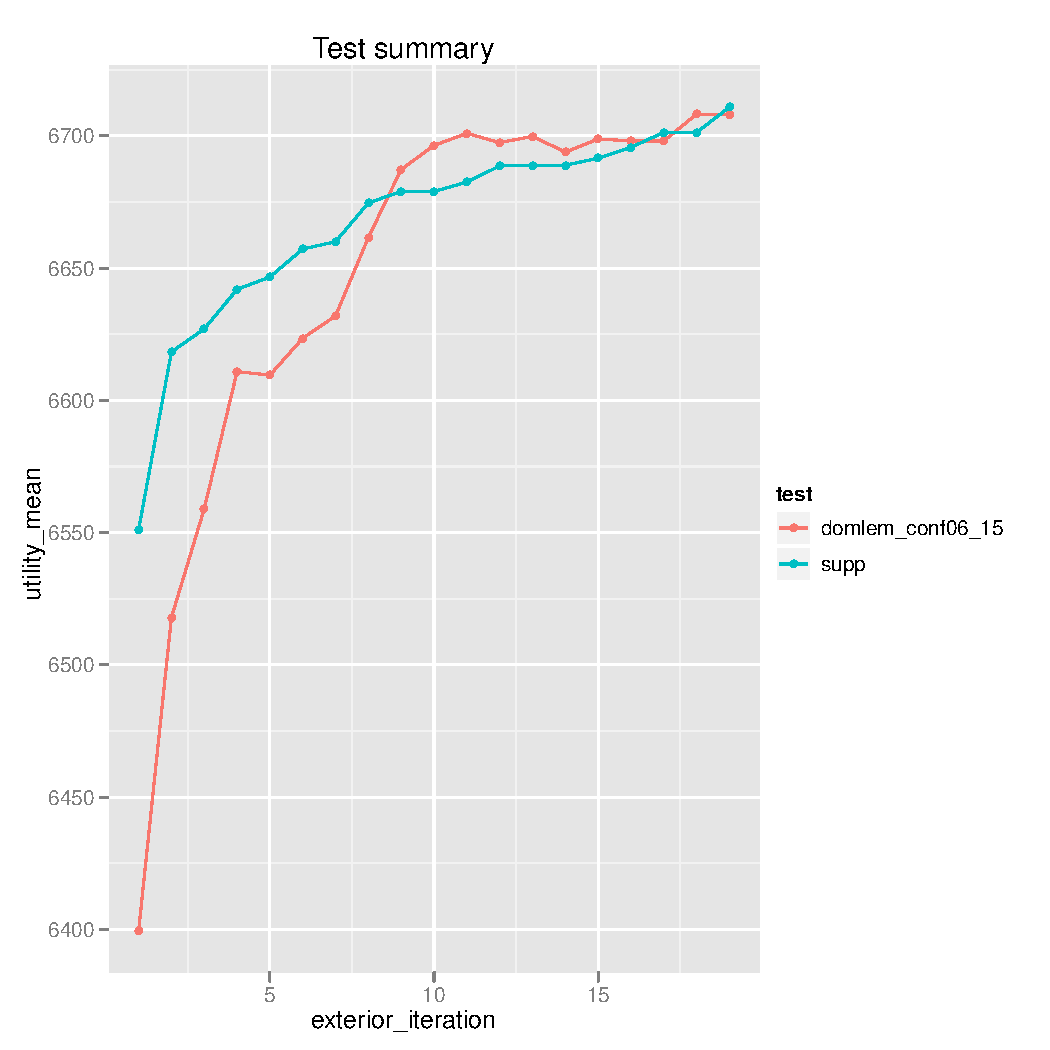
\includegraphics[scale=0.53]{exp/uncert/best/presentation}
      \label{pres_best1}
    }
    \subfloat{
      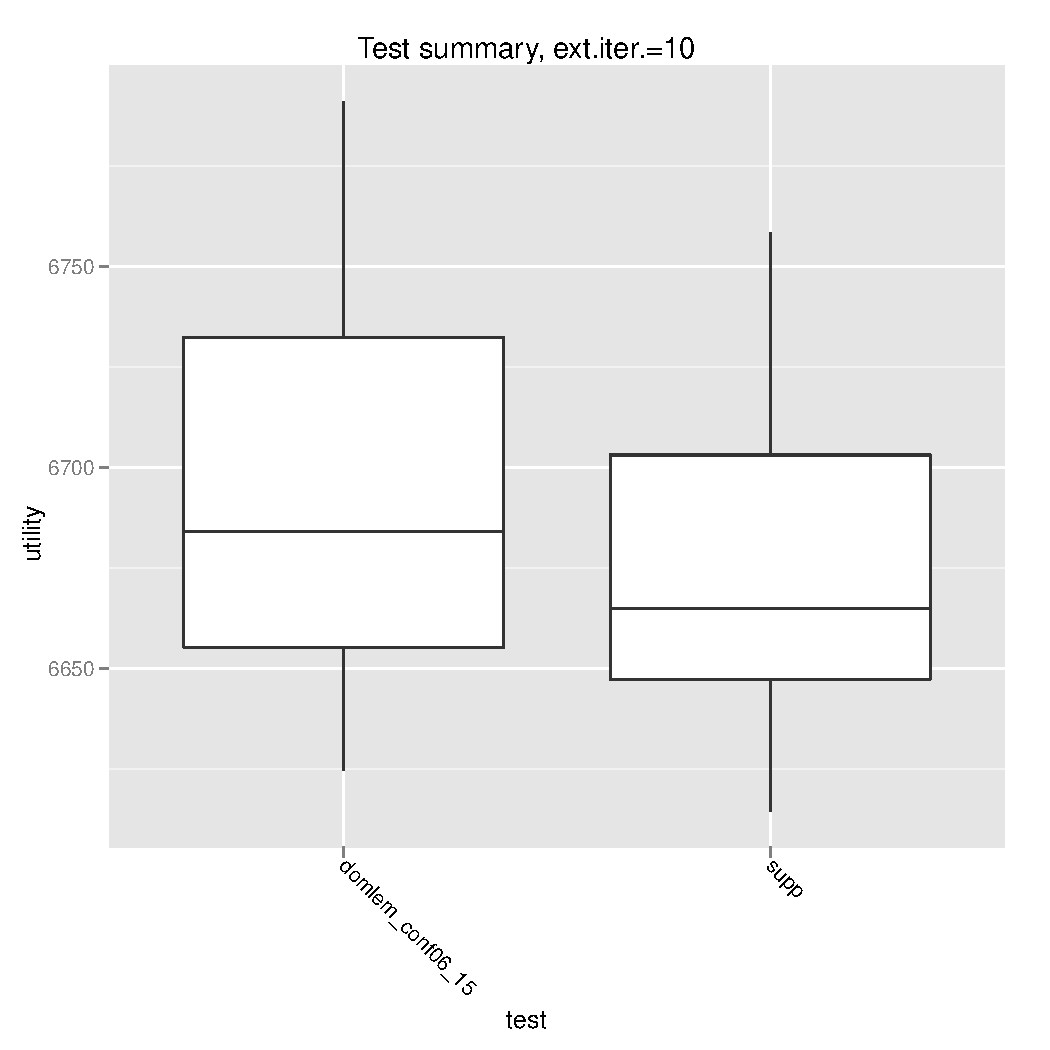
\includegraphics[scale=0.53]{exp/uncert/best/presentationb}
      \label{pres_best1b}
    }
  }
  \caption{Best runs for the mix problem}
  \label{pres_best}
\end{figure}

\begin{figure}
  \centering
  \makebox[\textwidth]{
    \subfloat{
      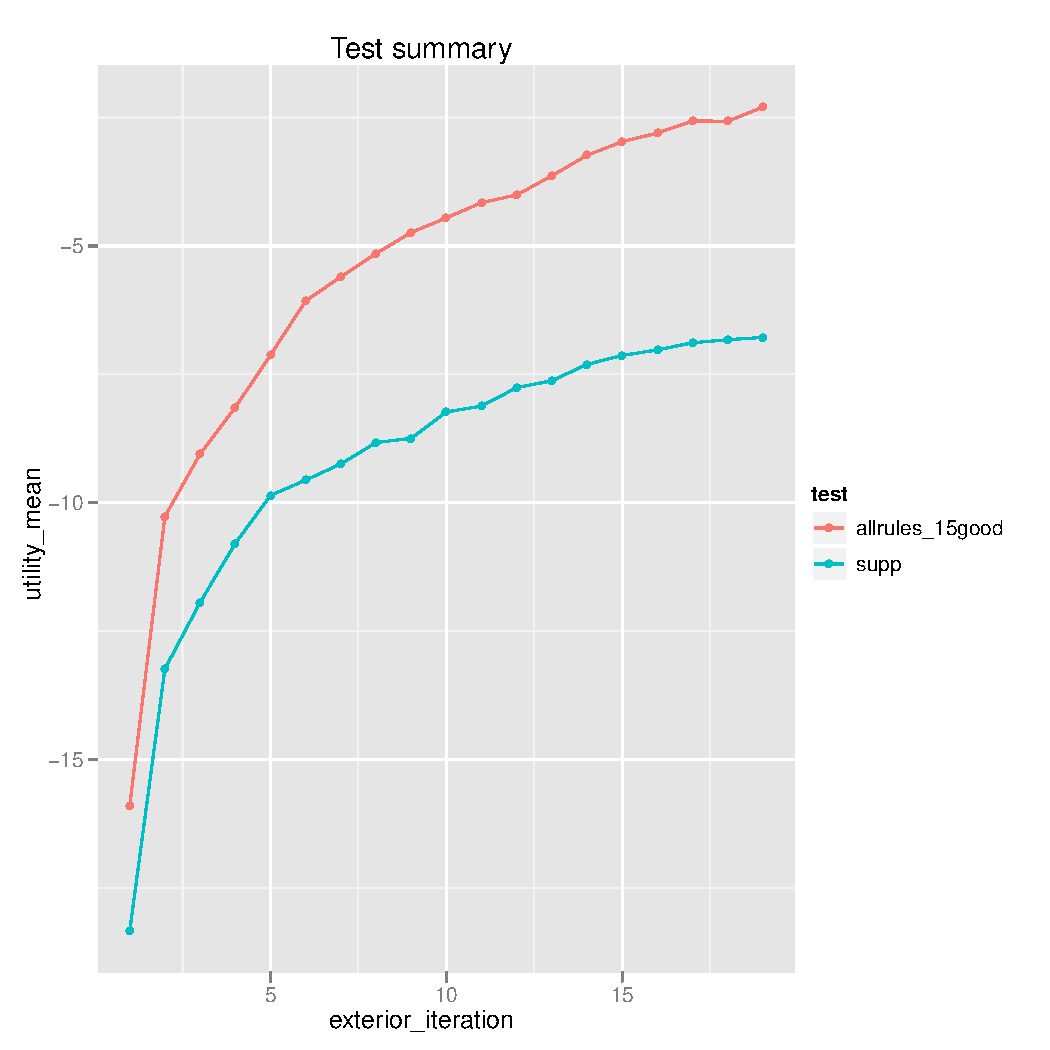
\includegraphics[scale=0.53]{exp/uncert/best/dtlz1_c4}
      \label{dtlz1_c4_best1}
    }
    \subfloat{
      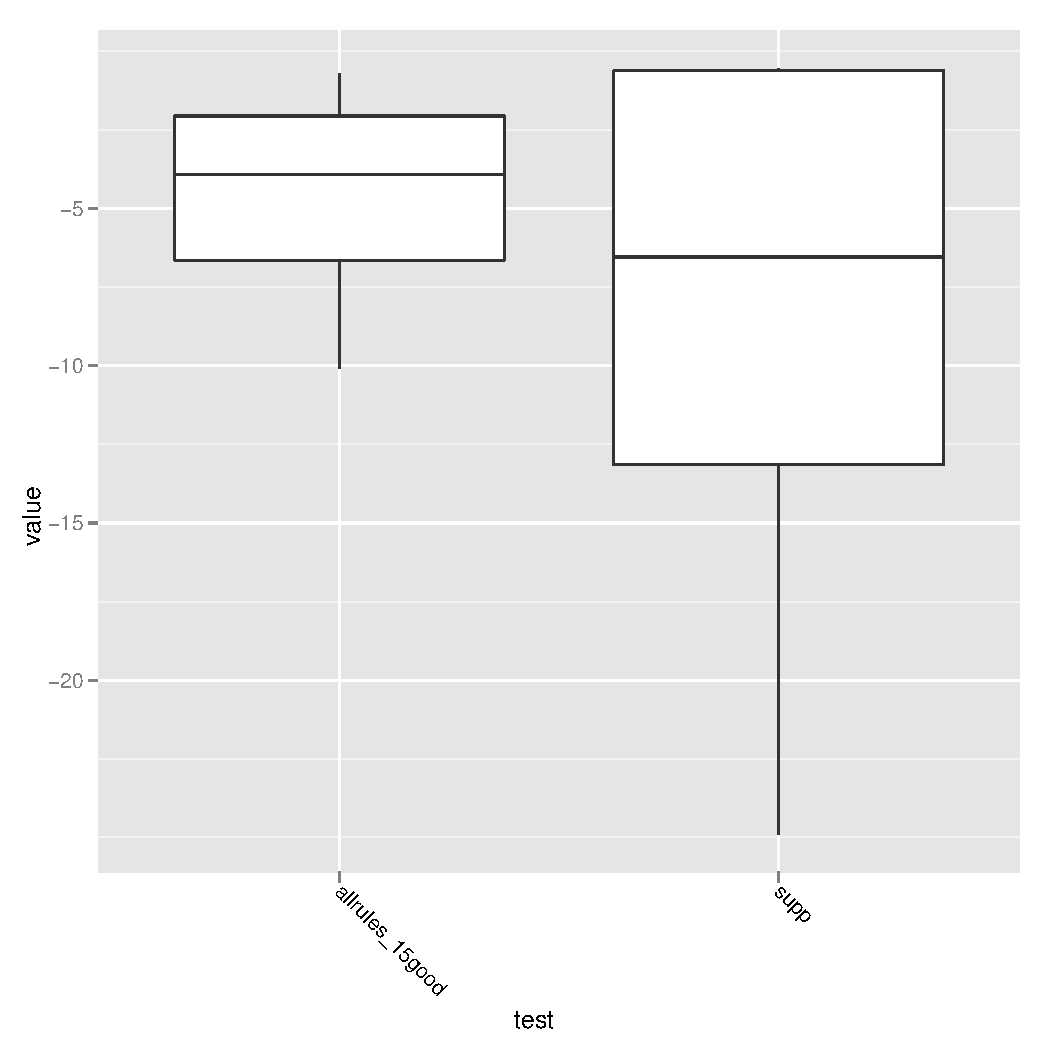
\includegraphics[scale=0.53]{exp/uncert/best/dtlz1_c4b}
      \label{dtlz1_c4_best1b}
    }
  }
  \caption{Best runs for the four-criteria DTLZ1 problem}
  \label{dtlz1_c4_best}
\end{figure}

\begin{figure}
  \centering
  \makebox[\textwidth]{
    \subfloat{
      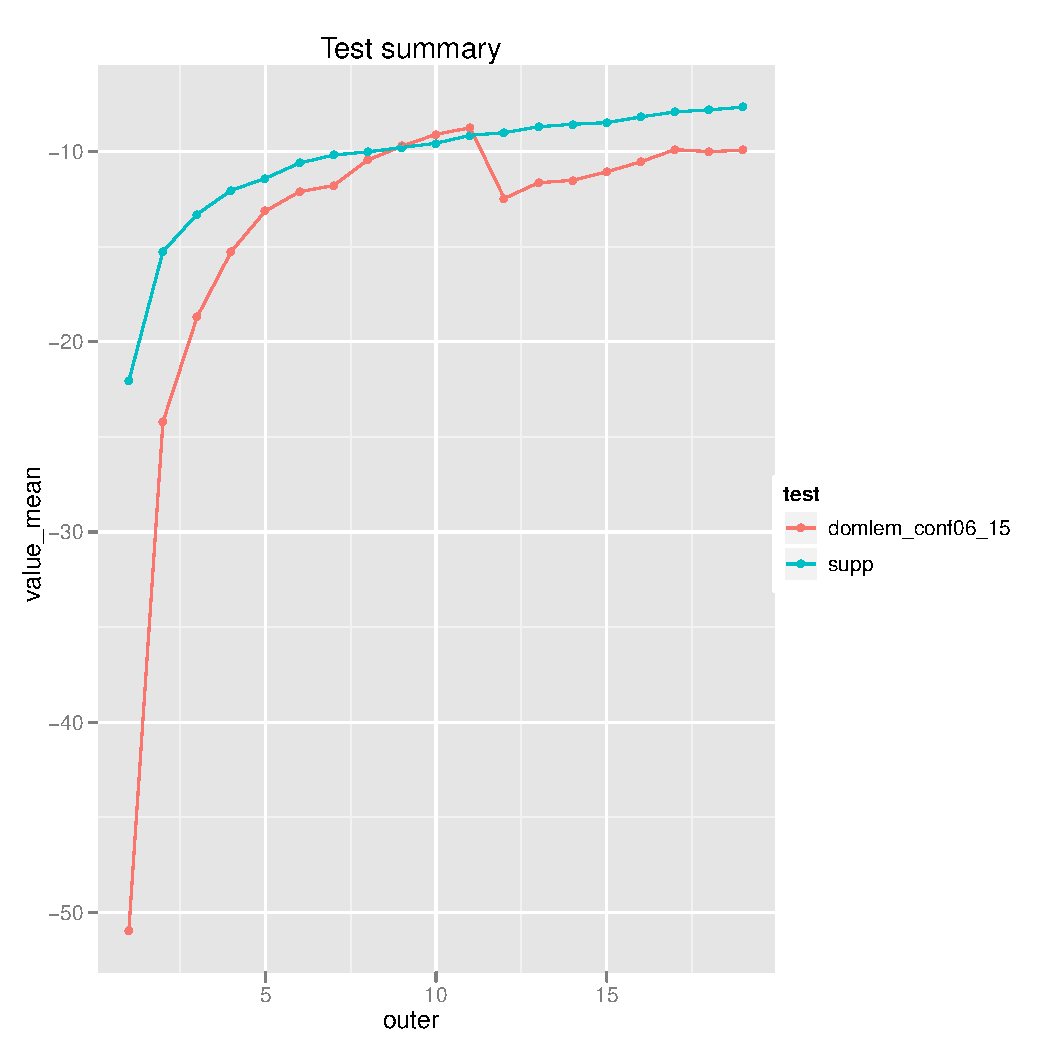
\includegraphics[scale=0.53]{exp/uncert/best/dtlz1_c10}
      \label{dtlz1_c10_best1}
    }
    \subfloat{
      \includegraphics[scale=0.53]{exp/uncert/best/dtlz1_c10b}
      \label{dtlz1_c10_best1b}
    }
  }
  \caption{Best runs for the ten-criteria DTLZ1 problem}
  \label{dtlz1_c10_best}
\end{figure}

\begin{figure}
  \centering
  \makebox[\textwidth]{
    \subfloat{
      \includegraphics[scale=0.53]{exp/uncert/best/dtlz7_c4}
      \label{dtlz7_c4_best1}
    }
    \subfloat{
      \includegraphics[scale=0.53]{exp/uncert/best/dtlz7_c4b}
      \label{dtlz7_c4_best1b}
    }
  }
  \caption{Best runs for the four-criteria DTLZ7 problem}
  \label{dtlz7_c4_best}
\end{figure}

\clearpage{}
%%% Local Variables: 
%%% mode: latex
%%% TeX-master: "main"
%%% End: 
